\documentclass[11pt,a4paper]{article}
\usepackage[utf8]{inputenc}
\usepackage[T1]{fontenc}
\usepackage{lmodern}
\usepackage[margin=1in]{geometry}
\usepackage{amsmath,amssymb,amsthm}
\usepackage{booktabs}
\usepackage{graphicx}
\usepackage{microtype}
\usepackage[numbers,sort&compress]{natbib}
\usepackage{xcolor}
\usepackage[colorlinks=true,linkcolor=blue!50!black,citecolor=blue!50!black,urlcolor=blue!50!black]{hyperref}
\usepackage{enumitem}
\usepackage{array}
\usepackage{caption}
\captionsetup{font=small,labelfont=bf}
\renewcommand{\topfraction}{0.9}
\renewcommand{\textfraction}{0.07}
\renewcommand{\floatpagefraction}{0.75}

\IfFileExists{numbers.tex}{% generated by experiments/make_numbers.py -- do not edit
\newcommand{\MetaSeed}{20260930}
\newcommand{\MetaPython}{3.11.15}
\newcommand{\MetaNumpy}{2.4.6}
\newcommand{\MetaScipy}{1.17.1}
\newcommand{\MetaSklearn}{1.9.1}
\newcommand{\MetaSeconds}{644}
\newcommand{\EoneConfigs}{500}
\newcommand{\EoneSettings}{8}
\newcommand{\EoneTotalConfigs}{4000}
\newcommand{\EoneBetweenTotal}{0}
\newcommand{\EoneCongTotal}{0}
\newcommand{\EoneGridExp}{30}
\newcommand{\EtwoMedDtwoNeight}{\ensuremath{8.6\times 10^{-3}}}
\newcommand{\EtwoMaxDtwoNeight}{\ensuremath{2.6\times 10^{-1}}}
\newcommand{\EtwoMedDtwoNsixteen}{\ensuremath{9.7\times 10^{-5}}}
\newcommand{\EtwoMaxDtwoNsixteen}{\ensuremath{3.5\times 10^{-4}}}
\newcommand{\EtwoMedDtwoNthirtytwo}{\ensuremath{4.6\times 10^{-6}}}
\newcommand{\EtwoMaxDtwoNthirtytwo}{\ensuremath{9.2\times 10^{-6}}}
\newcommand{\EtwoMedDtwoNsixtyfour}{\ensuremath{4.1\times 10^{-7}}}
\newcommand{\EtwoMaxDtwoNsixtyfour}{\ensuremath{7.4\times 10^{-7}}}
\newcommand{\EtwoMedDtwoNonetwentyeight}{\ensuremath{7.8\times 10^{-8}}}
\newcommand{\EtwoMaxDtwoNonetwentyeight}{\ensuremath{1.0\times 10^{-7}}}
\newcommand{\EtwoMedDtwoNtwofiftysix}{\ensuremath{2.7\times 10^{-8}}}
\newcommand{\EtwoMaxDtwoNtwofiftysix}{\ensuremath{3.7\times 10^{-8}}}
\newcommand{\EtwoMedDthreeNeight}{\ensuremath{4.3\times 10^{-2}}}
\newcommand{\EtwoMaxDthreeNeight}{\ensuremath{1.9\times 10^{-1}}}
\newcommand{\EtwoMedDthreeNsixteen}{\ensuremath{4.3\times 10^{-4}}}
\newcommand{\EtwoMaxDthreeNsixteen}{\ensuremath{8.0\times 10^{-4}}}
\newcommand{\EtwoMedDthreeNthirtytwo}{\ensuremath{1.1\times 10^{-5}}}
\newcommand{\EtwoMaxDthreeNthirtytwo}{\ensuremath{2.6\times 10^{-5}}}
\newcommand{\EtwoMedDthreeNsixtyfour}{\ensuremath{1.1\times 10^{-6}}}
\newcommand{\EtwoMaxDthreeNsixtyfour}{\ensuremath{1.3\times 10^{-6}}}
\newcommand{\EtwoMedDthreeNonetwentyeight}{\ensuremath{2.2\times 10^{-7}}}
\newcommand{\EtwoMaxDthreeNonetwentyeight}{\ensuremath{3.0\times 10^{-7}}}
\newcommand{\EtwoRepsDtwo}{30}
\newcommand{\EtwoRepsDthree}{15}
\newcommand{\EtwoNmaxDtwo}{256}
\newcommand{\EtwoNmaxDthree}{128}
\newcommand{\EtwoMedDtwoFirst}{\ensuremath{8.6\times 10^{-3}}}
\newcommand{\EtwoMedDtwoLast}{\ensuremath{2.7\times 10^{-8}}}
\newcommand{\EtwoMaxDtwoLast}{\ensuremath{3.7\times 10^{-8}}}
\newcommand{\EtwoMedDthreeFirst}{\ensuremath{4.3\times 10^{-2}}}
\newcommand{\EtwoMedDthreeLast}{\ensuremath{2.2\times 10^{-7}}}
\newcommand{\EtwoTotalRuns}{255}
\newcommand{\EtwoBn}{64}
\newcommand{\EtwoBreps}{20}
\newcommand{\EtwoBpreserved}{20}
\newcommand{\EtwoBmetricTrue}{\ensuremath{5.8\times 10^{-9}}}
\newcommand{\EtwoBmetricDist}{\ensuremath{4.5\times 10^{-2}}}
\newcommand{\EtwoBmetricDistMin}{\ensuremath{1.3\times 10^{-2}}}
\newcommand{\EtwoBordMax}{\ensuremath{4.3\times 10^{-31}}}
\newcommand{\EthreePatternsDone}{120}
\newcommand{\EthreeLeastDone}{994}
\newcommand{\EthreePatternsDtwo}{720}
\newcommand{\EthreeLeastDtwo}{53}
\newcommand{\EthreePatternsDthree}{720}
\newcommand{\EthreeLeastDthree}{81}
\newcommand{\EthreeSamples}{300\,000}
\newcommand{\EthreeTriAnglesA}{36.9, 53.1, 90.0}
\newcommand{\EthreeTriAnglesB}{26.4, 36.3, 117.3}
\newcommand{\EfourTrials}{300}
\newcommand{\EfourN}{30}
\newcommand{\EfourAffMono}{0.35}
\newcommand{\EfourGabrielMono}{0.03}
\newcommand{\EtwoSlopeDtwo}{2.9}
\newcommand{\EtwoSlopeDthree}{3.6}
\newcommand{\EfiveAn}{300}
\newcommand{\EfiveAtrials}{200}
\newcommand{\EfiveAconfPreserved}{200}
\newcommand{\EfiveAconfTauChange}{23}
\newcommand{\EfiveAboostPreserved}{200}
\newcommand{\EfiveAboostTauChange}{\ensuremath{10^{-9}}}
\newcommand{\EfiveArotChanged}{19.6}
\newcommand{\EfiveArotChangedMin}{5.9}
\newcommand{\EfiveBn}{400}
\newcommand{\EfiveBreps}{60}
\newcommand{\EfiveCnmin}{250}
\newcommand{\EfiveCnmax}{2000}
\newcommand{\EfiveCpairsTotal}{39\,000}
\newcommand{\EfiveCcorrLast}{0.990}
\newcommand{\EfiveCcorrDistLast}{0.91}
\newcommand{\EfiveCslopeFirst}{1.73}
\newcommand{\EfiveCslopeLast}{1.85}
\newcommand{\EfiveCerrFirst}{14}
\newcommand{\EfiveCerrLast}{8}
\newcommand{\EfiveCerrDistLast}{17}
\newcommand{\EfiveCerrDistFirst}{23}
\newcommand{\EfiveDnmin}{250}
\newcommand{\EfiveDnmax}{2000}
\newcommand{\EfiveDrmseFirst}{0.073}
\newcommand{\EfiveDrmseLast}{0.031}
\newcommand{\EfiveDsqrtFirst}{1.15}
\newcommand{\EfiveDsqrtLast}{1.40}
\newcommand{\EfiveDdisagreeLast}{3.69}
\newcommand{\EfiveSeconds}{15}
\newcommand{\HasLorentz}{1}
}{}
\providecommand{\HasLorentz}{0}
\providecommand{\HasClass}{0}
\providecommand{\HasRlaw}{0}
\providecommand{\HasRlawChk}{0}
\providecommand{\HasSharp}{0}
\providecommand{\HasSecond}{0}

\theoremstyle{plain}
\newtheorem{theorem}{Theorem}[section]
\newtheorem{proposition}[theorem]{Proposition}
\newtheorem{lemma}[theorem]{Lemma}
\newtheorem{corollary}[theorem]{Corollary}
\theoremstyle{definition}
\newtheorem{definition}[theorem]{Definition}
\newtheorem{example}[theorem]{Example}
\newtheorem{claim}[theorem]{Claim}
\newtheorem{conjecture}[theorem]{Conjecture}
\theoremstyle{remark}
\newtheorem{remark}[theorem]{Remark}

\newcommand{\R}{\mathbb{R}}
\newcommand{\Obj}{\mathrm{Obj}}
\newcommand{\Inv}{\mathrm{Inv}}
\newcommand{\Sim}{\mathrm{Sim}}
\newcommand{\Euc}{\mathrm{E}}
\newcommand{\Fcoord}{\mathsf{Coord}}
\newcommand{\Fmet}{\mathsf{Met}}
\newcommand{\Ford}{\mathsf{Ord}}
\newcommand{\Frel}{\mathsf{Rel}}
\newcommand{\Fcaus}{\mathsf{Caus}}
\newcommand{\Fcausn}{\mathsf{Caus}{+}\mathsf{N}}
\newcommand{\ord}{\preccurlyeq}
\newcommand{\incomp}{\parallel}
\newcommand{\dd}{\mathrm{d}}
\newcommand{\status}[1]{\textsf{\small [#1]}}

\title{\textbf{Foundational Geometry:}\\[2pt]
\large Invariants Across Formalisms and Structures Preceding a Geometric Description}
\author{Luciano Silva Alarco\\
\small Pontificia Universidad Cat\'olica del Per\'u\\
\small ORCID 0000-0002-3395-3129}
\date{\small Working draft v0.8 --- research line MRT001 --- 3 October 2026}

\begin{document}
\maketitle

\begin{abstract}
\noindent
We ask which claims about ``structures that precede a geometric description'' can be formulated and tested inside explicitly defined mathematical frameworks. We introduce a minimal bookkeeping language: a \emph{formalism} is a class of structures, a \emph{translation} is a map between formalisms, and an \emph{invariant across formalisms} is a quantity that factors through a translation. Geometry then appears as what survives the passage from a richer to a poorer formalism, in the spirit of Klein's Erlangen programme and of the meaningfulness criterion of measurement theory. The language is worked out in full on one chain where every step can be proved or computed, the finite Euclidean chain
\emph{coordinates} $\to$ \emph{distance matrix} $\to$ \emph{ranking of distances} $\to$ \emph{betweenness and congruence}. Three results are established. (i)~On generic finite samples the relational primitives of elementary geometry are empty: exact integer arithmetic over \EoneTotalConfigs{} random configurations produced no non-degenerate instance of betweenness or congruence, while integer grids produce dozens to thousands; the primitives that axiomatise the continuum are therefore not sample-robust. (ii)~The ordinal formalism is strictly coarser than similarity geometry for every finite $n\ge 3$, yet a non-metric reconstruction from the ranking alone recovers the configuration up to similarity with a median Procrustes disparity of \EtwoMedDtwoLast{} at $n=\EtwoNmaxDtwo$ in the plane, \EtwoDropDtwo{} orders of magnitude below its value at $n=8$; this is the finite-sample face of the asymptotic uniqueness theorem for ordinal embeddings, and the class itself is measured directly: its inradius, in the norm $\max_i\lVert y_i-x_i\rVert$, lies between a quarter and a half of the minimal gap between consecutive sorted distances (exactly a quarter when the two extremal pairs are disjoint), a quantity that scales empirically as $n^{-\EtwocSlopeGap}$. (iii)~Standard geometric quantities sort themselves by \emph{formalism depth}: minimum spanning tree, nearest-neighbour graph, relative neighbourhood graph and diameter pair are ordinal invariants, whereas diameter, affine dimension and the Gabriel graph are metric but not ordinal invariants at finite $n$. The same language is then applied to the causal-order translation \emph{Lorentzian coordinates} $\to$ \emph{causal order}, followed by a statistical step that adds counting, on uniform sprinklings of the $1{+}1$ Minkowski diamond, where the kernel of the order translation contains the conformal group and coincides with it for some but not all finite configurations, and counting restores proper times and coordinates. We prove that the number of realizers of the causal order of a uniform sample, that is, the number of conformal orbits, up to parity, that make up its kernel class, converges in law to $2^{Z}$ with $Z$ Poisson of mean one, at rate $O(1/n)$, and we identify the exceptions to the equality with $2^{N}$, $N$ the number of descending successions of the permutation that sends $u$-ranks to $v$-ranks; the proof is self-contained except for Gallai's theorem on prime comparability graphs, and the combinatorial lemmas it uses are known and reproved. We also identify the first-order term: the total variation distance to $2^Z$ is $(1+1/(2e))/n+O(n^{-2})$, a result checked by an independent internal referee; in this version, and not yet refereed, we make the remainder explicit (at most $\SecCtwentytwo/n^2$ for $n\ge22$) and show that the number of descending successions is at total variation distance $(3/(4e)+o(1))/n^2$ from $\mathrm{Po}(1-1/n)$, while the $n^{-2}$ term of the realizer law is only computed, from the exact law, and its closed form is conjectural. The paper claims no unified theory and reports no experimental physics; its contribution is to turn a recurring foundational phrase into a list of statements with explicit status.
\end{abstract}

\section{Introduction}\label{sec:intro}

The idea that geometry is not primitive, that something poorer than a metric or a coordinate system comes first and geometry is recovered from it, is old and recurs in several disciplines under different names. Klein's Erlangen programme defines a geometry by the group of transformations under which its statements are invariant~\citep{klein1872}. Hilbert and Tarski axiomatise Euclidean geometry from the primitive relations of betweenness and congruence~\citep{hilbert1899,tarski1959,tarskigivant1999}. Menger and Blumenthal ask which metric spaces are ``Euclidean'' and how much of a configuration a distance table determines~\citep{menger1928,blumenthal1953}. Measurement theory calls a statement \emph{meaningful} when it is invariant under the admissible transformations of the scale on which the quantities were measured~\citep{stevens1946,krantz1971,narens2002}. In relativity, the causal order of a spacetime determines its topology and its conformal geometry~\citep{hawking1976,malament1977}, and the causal set programme~\citep{bombelli1987} condenses this, in Sorkin's later slogan, into ``order plus number equals geometry''~\citep{sorkin2005}.

Each of these traditions is precise on its own ground, but the phrase ``structure preceding geometry'' is often used across them without saying which structure, which geometry, and in what sense one precedes the other. The research line to which this draft belongs (MRT001) had, at the time of writing, the modest and explicit objective of \emph{specifying which claims of this kind can be formulated and tested within defined mathematical frameworks}. This paper is an attempt to discharge that objective by three moves.

\begin{enumerate}[leftmargin=2em]
\item We introduce a small bookkeeping language (Section~\ref{sec:language}): formalisms, translations between them, the kernel of a translation, invariants along a translation, and the \emph{formalism depth} of a quantity. Nothing in it is new; its purpose is to make ``$G$ precedes $F$'' a predicate that can be checked.
\item We work the language out completely on one chain where every claim can be proved or computed: finite configurations of points in $\R^d$, read successively as coordinates, as a distance matrix, as a ranking of the pairwise distances, and as Tarski's betweenness and congruence relations (Sections~\ref{sec:euclid} and~\ref{sec:depth}).
\item We apply the same language to the causal order of a uniform sprinkling of $1{+}1$ Minkowski space (Section~\ref{sec:lorentz}), where the continuum theorems of Hawking--King--McCarthy and Malament have finite, computable counterparts, and where the finite-$n$ ambiguity of the order obeys an exact limit law (Theorem~\ref{thm:realizers}).
\end{enumerate}

\paragraph{Scope.} We do not propose a unified theory, a new geometry or a physical model; the Lorentzian part is a mathematical model with a fixed background and is used only because it is the sharpest known instance of ``order before metric''. Every numerical statement in the paper is produced by four short scripts included with the manuscript, with a fixed seed, and by three more that check the proofs of Section~\ref{sec:lorentz} numerically (Appendices~\ref{app:repro} and~\ref{app:realizers}). Section~\ref{sec:claims} lists all claims with their status: proved here, classical, taken from the literature, computationally verified, or conjectural.

\section{Formalisms, translations and invariants}\label{sec:language}

\begin{definition}[Formalism]
A \emph{formalism} is a pair $F=(\Obj_F,\cong_F)$ consisting of a class of objects and an equivalence relation on it, read as isomorphism. Two objects that are isomorphic are regarded as the same description.
\end{definition}

\begin{definition}[Translation, kernel]
A \emph{translation} $\tau\colon F\to G$ is a map $\Obj_F\to\Obj_G$ such that $X\cong_F Y$ implies $\tau X\cong_G \tau Y$. Its \emph{kernel} is the equivalence relation $X\sim_\tau Y \iff \tau X\cong_G \tau Y$ on $\Obj_F$, which is coarser than (contains) $\cong_F$. Two objects in the same kernel class are \emph{indistinguishable in $G$}.
\end{definition}

\begin{definition}[Invariant across formalisms]
A function $\Phi$ on $\Obj_F$ is an \emph{invariant along $\tau$}, or a $G$-invariant of $F$, if $X\sim_\tau Y$ implies $\Phi(X)=\Phi(Y)$; equivalently, $\Phi$ factors through $\tau$. We write $\Inv(\tau)$ for the set of such functions.
\end{definition}

\begin{definition}[Chain, formalism depth]\label{def:chain}
A \emph{chain} is a sequence of translations $F_0\xrightarrow{\tau_1}F_1\xrightarrow{\tau_2}\cdots\xrightarrow{\tau_k}F_k$. The \emph{formalism depth} of a quantity $\Phi$ on $\Obj_{F_0}$ is the largest $i$ such that $\Phi\in\Inv(\tau_i\circ\cdots\circ\tau_1)$, that is, the poorest formalism in the chain from which $\Phi$ can still be computed; the empty composition ($i=0$) is allowed, so a quantity that is not invariant even along $\tau_1$ has depth $0$, the coordinate level.
\end{definition}

\begin{lemma}[Monotonicity]\label{lem:mono}
For composable translations, $\Inv(\tau_2\circ\tau_1)\subseteq\Inv(\tau_1)$. Hence along a chain the sets of invariants decrease and the kernels increase.
\end{lemma}
\begin{proof}
If $\tau_1X\cong\tau_1Y$ then $\tau_2\tau_1X\cong\tau_2\tau_1Y$, so $\sim_{\tau_1}\subseteq\sim_{\tau_2\tau_1}$, and a function constant on the classes of the coarser relation is constant on those of the finer one.
\end{proof}

\begin{definition}[Faithfulness, precedence]
Let $\tau\colon F\to G$ and let $\mathcal C\subseteq\Obj_F$ be a class of objects of interest. The translation is \emph{faithful on $\mathcal C$ up to a group $H$} acting on $\Obj_F$ if, for $X,Y\in\mathcal C$, $X\sim_\tau Y$ implies $Y=hX$ for some $h\in H$. For a family of formalisms $F_n$ (below, $\Fcoord(n,d)$), classes $\mathcal C_n\subseteq\Obj_{F_n}$ and a fixed $H$-invariant distance $\delta$ on $\Obj_{F_n}$ (below, the Procrustes disparity), translations $\tau_n$ are \emph{asymptotically faithful up to $H$} on $(\mathcal C_n)$ if $\sup\{\delta(X,Y): X\in\mathcal C_n,\ Y\sim_{\tau_n}X\}\to0$ as $n\to\infty$. We say that $G$ \emph{precedes} $F$ on $\mathcal C$ when $\tau$ has a non-trivial kernel and is nevertheless faithful, or asymptotically faithful, up to a group $H$ that is itself a symmetry group of $F$.
\end{definition}

The definition makes the foundational phrase testable: to claim that a structure $G$ precedes a geometry $F$ one must exhibit the translation, compute or bound its kernel, and prove or measure its faithfulness. Two classical readings are recovered at once.

\begin{remark}[Erlangen]
If $\Obj_F$ is a set with an action of a group $H$ and $\tau$ is the quotient map to $\Obj_F/H$, then $\Inv(\tau)$ is exactly the set of $H$-invariants, Klein's geometry of the pair $(\Obj_F,H)$. Euclidean, similarity, affine and projective geometry are the invariants of successively coarser quotients, and Lemma~\ref{lem:mono} is the Erlangen hierarchy.
\end{remark}

\begin{remark}[Meaningfulness]
Stevens' scale types are kernels of translations~\citep{stevens1946}. A ratio scale identifies quantities up to a positive factor, an interval scale up to a positive affine map, an ordinal scale up to a monotone bijection. A statement is \emph{meaningful} in the sense of \citet{krantz1971} and \citet{narens2002} precisely when it is an invariant along the corresponding translation. The chain studied below realises two of these scale types on one object: the distance matrix is a ratio-scale description of a configuration and the ranking of distances is its ordinal-scale description; a configuration read up to similarity is what the ratio scale determines.
\end{remark}

\section{The finite Euclidean chain}\label{sec:euclid}

Fix $n\ge 3$ and $d\ge 1$. Write $[n]=\{1,\dots,n\}$ and $P_n$ for the set of unordered pairs of distinct elements of $[n]$, $m=|P_n|=\binom n2$. All objects are labelled; quotienting by relabelling adds a graph-isomorphism layer that is orthogonal to the questions asked here.

\begin{itemize}[leftmargin=2em]
\item $\Fcoord(n,d)$: injective configurations $X=(x_1,\dots,x_n)\in(\R^d)^n$ (distinct points), with equality as isomorphism.
\item $\Fmet(n)$: symmetric matrices $D\in\R^{n\times n}$ with zero diagonal and positive off-diagonal entries, with equality as isomorphism.
\item $\Ford(n)$: total preorders $\ord$ on $P_n$ (generically total orders), with equality as isomorphism.
\item $\Frel(n)$: pairs $(B,C)$ of a ternary relation $B\subseteq[n]^3$ (betweenness) and a binary relation $C\subseteq P_n\times P_n$ (congruence), with equality as isomorphism.
\end{itemize}

The translations are the obvious ones. $\tau_1\colon\Fcoord\to\Fmet$ sends $X$ to its distance matrix $D_X=(\lVert x_a-x_b\rVert)_{a,b}$. $\tau_2\colon\Fmet\to\Ford$ sends $D$ to the preorder $\{a,b\}\ord\{c,d\}\iff D_{ab}\le D_{cd}$. $\tau_3\colon\Fmet\to\Frel$ sends $D$ to
\[
B_D=\{(a,b,c)\ \text{distinct}: D_{ab}+D_{bc}=D_{ac}\},\qquad
C_D=\{(p,q)\in P_n^2: p\ne q,\ D_p=D_q\}.
\]
The congruence part of $\tau_3$ factors through $\tau_2$ (congruent pairs are ties of the preorder) but the betweenness part does not, since it involves an additive equality; the chain therefore branches at $\Fmet$.

\subsection{Coordinates to metric: the classical step}

\begin{theorem}[Schoenberg; Young and Householder]\label{thm:classical}
Two labelled configurations $X,Y\in(\R^d)^n$ have the same distance matrix if and only if $Y=gX$ for a Euclidean motion $g\in\Euc(d)$, possibly improper. A matrix $D$ is the distance matrix of a configuration in $\R^d$ if and only if $-\tfrac12 J D^{(2)} J$ is positive semidefinite of rank at most $d$, where $D^{(2)}$ is the entrywise square and $J=I-\tfrac1n\mathbf 1\mathbf 1^{\!\top}$.
\end{theorem}
\noindent See \citet{schoenberg1935,younghouseholder1938,blumenthal1953}. In the language of Section~\ref{sec:language}: $\ker\tau_1$ is the orbit relation of $\Euc(d)$, $\tau_1$ is faithful up to $\Euc(d)$ on all of $\Fcoord$, and $\Inv(\tau_1)$ is Euclidean geometry in Klein's sense. The metric formalism precedes the coordinate one in the strongest possible way: nothing is lost except position and orientation.

\subsection{Metric to relations: the primitives are empty on samples}

Tarski's system axiomatises elementary Euclidean geometry with the single sort ``point'' and the two primitives betweenness and congruence, and the system is complete and decidable~\citep{tarski1959,tarskigivant1999}. The restriction of these primitives to a finite sample behaves very differently from their behaviour on the continuum.

\begin{proposition}[Generic emptiness]\label{prop:empty}
Let $d\ge 2$ and $n\ge 3$, and let $\mathcal G\subseteq(\R^d)^n$ be the set of configurations in which no three points are collinear and all $m$ pairwise distances are distinct. Then $\mathcal G$ is open, dense and of full Lebesgue measure, and for every $X\in\mathcal G$
\[
B_{D_X}=\varnothing\qquad\text{and}\qquad C_{D_X}=\varnothing .
\]
Consequently $\tau_3\circ\tau_1$ is constant on $\mathcal G$: its kernel identifies all generic configurations of a given size, and every relational invariant is constant on $\mathcal G$.
\end{proposition}
\begin{proof}
Collinearity of three distinct points $x_a,x_b,x_c$ is the vanishing of all $2\times 2$ minors of the $d\times 2$ matrix $[\,x_b-x_a\mid x_c-x_a\,]$, a system of polynomial equations in the coordinates that is not identically satisfied when $d\ge2$; its solution set is a proper real-algebraic subset, hence closed, nowhere dense and null. Equality $\lVert x_a-x_b\rVert^2=\lVert x_c-x_d\rVert^2$ for two distinct pairs is a single non-constant polynomial equation (non-constant because moving $x_a$ alone changes the left side and, when $a\notin\{c,d\}$, not the right; when the pairs share a point the same argument applies to the point that is not shared), with the same consequences. $\mathcal G$ is the complement of a finite union of such sets, so it is open, dense and of full measure. For $X\in\mathcal G$: if $D_{ab}+D_{bc}=D_{ac}$ with $a,b,c$ distinct then, by the equality case of the triangle inequality for the Euclidean norm (strict convexity), $x_b-x_a$ and $x_c-x_b$ are non-negative multiples of one another, so $x_b$ lies on the segment $[x_a,x_c]$ and the three points are collinear, contradicting $X\in\mathcal G$. A congruence $(p,q)$ with $p\ne q$ contradicts distinctness of the distances. The final assertion follows because $\tau_3\tau_1 X=(\varnothing,\varnothing)$ for all $X\in\mathcal G$.
\end{proof}

\begin{remark}[The line]
For $d=1$ every triple is collinear and $B_{D_X}$ is the betweenness relation of the linear order of the sample, which is far from empty; the proposition then holds only for $C$. On the line the relational formalism carries exactly the order type of the sample, which is the structure Section~\ref{sec:lorentz} takes as its starting point.
\end{remark}

\paragraph{Computational check (E1).}
Proposition~\ref{prop:empty} is a statement about a full-measure set, and a floating-point test of the equalities defining $B$ and $C$ would be misleading: the betweenness gap $D_{ab}+D_{bc}-D_{ac}$ is quadratic in the distance from $x_b$ to the line through $x_a,x_c$, so a relative tolerance of $10^{-9}$ admits every triple whose middle point lies within about $10^{-4.5}$ of a line and, at $n=50$, produced of the order of one spurious triple per configuration in a preliminary floating-point run. We therefore sample integer coordinates uniformly in $\{0,\dots,2^{\EoneGridExp}-1\}^d$ and test collinearity and equality of squared distances \emph{exactly} in 64-bit integer arithmetic (the sampling grid is fine enough that the result is the generic one with overwhelming probability, and coarse enough that an exact coincidence, should one occur, would be counted). Table~\ref{tab:e1} reports the totals: across \EoneSettings{} settings and \EoneTotalConfigs{} configurations, \EoneBetweenTotal{} betweenness instances and \EoneCongTotal{} congruence instances were found. The integer grids in the lower panel, where the relations are rich, show that the test itself is not blind.

\begin{table}[t]
\centering\small
\begin{tabular}{rrrrr}
\toprule
$n$ & $d$ & configurations & betweenness instances & congruence instances\\
\midrule
5 & 2 & 500 & 0 & 0 \\
10 & 2 & 500 & 0 & 0 \\
20 & 2 & 500 & 0 & 0 \\
50 & 2 & 500 & 0 & 0 \\
5 & 3 & 500 & 0 & 0 \\
10 & 3 & 500 & 0 & 0 \\
20 & 3 & 500 & 0 & 0 \\
50 & 3 & 500 & 0 & 0
\\
\midrule
\multicolumn{2}{l}{grid} & $n$ & betweenness instances & congruence instances\\
\midrule
3$\times$3 & 9 & 8 & 138 \\
4$\times$4 & 16 & 44 & 976 \\
5$\times$5 & 25 & 152 & 4242
\\
\bottomrule
\end{tabular}
\caption{E1. Exact counts of non-degenerate betweenness triples and congruent pair-pairs in random integer configurations (upper panel, \EoneConfigs{} configurations per row) and in square integer grids (lower panel). A betweenness instance is a pair $(b,\{a,c\})$ with $b$ strictly between $a$ and $c$ (a row of four collinear points contributes $1+1+2=4$); a congruence instance is an unordered pair of distinct point-pairs at equal distance.}
\label{tab:e1}
\end{table}

\begin{remark}[Axiomatic versus observational primitives]
The primitives that make Tarski's theory complete on the plane carry no information about a generic finite sample of the plane. Any empirical test of a geometric claim uses finitely many measured points, so such a test must pass through the metric or the ordinal formalism; betweenness and congruence can only be \emph{inferred} from them, with a tolerance whose meaning depends on $n$ and on the chosen tolerance, not on the configuration. This is the first precise sense in which ``the structure that precedes geometry'' cannot be the axiomatic primitives.
\end{remark}

\subsection{Metric to ordinal: finite non-uniqueness}

\begin{proposition}[Finite non-uniqueness]\label{prop:nonunique}
Let $n\ge3$, $d\ge1$. For every configuration $X$ of distinct points whose pairwise distances are distinct, the kernel class of $X$ under $\tau_2\circ\tau_1$ contains a neighbourhood of $X$ in $(\R^d)^n$, and that neighbourhood contains configurations that are not similar to $X$. In particular $\tau_2\tau_1$ is not faithful up to $\Sim(d)$ on any open set, for any finite $n$.
\end{proposition}
\begin{proof}
The distances are continuous functions of $X$, and the ordinal pattern of $X$ is defined by finitely many strict inequalities between them, which persist in a neighbourhood $U$ of $X$; so $U$ lies in the kernel class. Pick three labels $a,b,c$ and move $x_b$ along the ray from $x_a$ through $x_b$ by a small amount: $D_{ab}$ changes while $D_{ac}$ does not, so the ratio $D_{ab}/D_{ac}$ changes. Similarities preserve all distance ratios, hence the moved configuration, which lies in $U$ for a small enough move, is not similar to $X$.
\end{proof}

\begin{example}[E3]\label{ex:e3}
On the line, $\{0,1,3\}$ and $\{0,1,2.5\}$ have the same ordinal pattern (distances $1<2<3$ and $1<1.5<2.5$ in the same pair order) and are not similar. In the plane, the triangles with sides $(3,4,5)$ and $(3,4,6)$ have the same pattern and angles $(\EthreeTriAnglesA)$ and $(\EthreeTriAnglesB)$ degrees respectively. For $n=3$ the ordinal formalism records exactly the order of the three sides, equivalently the order of the three angles, and its generic fibres are the six open cells into which these orderings cut the two-dimensional shape space of triangles.
\end{example}

The ordinal formalism nevertheless retains dimensional information. For $n=4$ there are $720$ possible orderings of the six distances. Sampling \EthreeSamples{} uniform configurations, we observe \EthreePatternsDone{} distinct orderings on the line but all \EthreePatternsDtwo{} in the plane and all \EthreePatternsDthree{} in space (the least frequent planar ordering was seen \EthreeLeastDtwo{} times, so the count is not an artefact of sample size). The count on the line has a short explanation: for sorted points with gaps $u,v,w$ the six distances are $u,v,w,u+v,v+w,u+v+w$, and only ten orderings of these are consistent with positivity, each labelled pattern arising from two (labelling, gap-order) combinations under reflection, giving $24\cdot10/2=120$.

\subsection{Metric to ordinal: asymptotic faithfulness}

\begin{theorem}[Kleindessner and von Luxburg; informal statement]\label{thm:kvl}
Let $\Omega\subset\R^d$ be bounded, connected and open and satisfy the mild regularity condition imposed in~\citet{kleindessner2014} (for instance, $\Omega$ a finite union of open balls), and let $x_1,x_2,\dots$ be points of $\Omega$ that become dense in $\Omega$. Then the complete ordinal pattern of $(x_1,\dots,x_n)$, that is, the outcome of \emph{all} comparisons $D_{ab}<D_{cd}$ over quadruples of labels, determines the configuration up to similarity in the limit: any sequence of configurations $y^{(n)}\in(\R^d)^n$, in the same dimension $d$, with the same ordinal pattern as $(x_1,\dots,x_n)$ converges, after alignment by similarity transformations, to the original points as $n\to\infty$, in the sense made precise in~\citet{kleindessner2014}.
\end{theorem}
\noindent We state the theorem informally and refer to the source for the exact regularity condition and for the mode of convergence. \citet{terada2014} obtain a conclusion of the same kind when only the unweighted $k$-nearest-neighbour graph of the sample is retained, for points drawn from a density on a suitable domain and $k\to\infty$ with $k/n\to0$, at a rate specified there. In our language, take $\mathcal C_n=\{(x_1,\dots,x_n)\}$, the initial segments of one fixed dense sequence, and $\delta$ the Procrustes disparity; the theorem, read with the alignment uniform over the labels $i\le n$, which is what a vanishing disparity requires, says that $\tau_2\tau_1$ is asymptotically faithful up to $\Sim(d)$ on $(\mathcal C_n)$. The ordinal formalism therefore precedes similarity geometry on dense samples of such domains, although by Proposition~\ref{prop:nonunique} it never does so exactly at finite $n$.

\paragraph{Computational check (E2).}
For $d\in\{2,3\}$ and $n$ from $8$ to $\EtwoNmaxDtwo$ ($\EtwoNmaxDthree$ for $d=3$) we sample $n$ points uniformly in the unit cube, compute the rank matrix of the pairwise distances (so that \emph{only} the ordinal pattern enters), reconstruct a configuration by non-metric multidimensional scaling~\citep{shepard1962,kruskal1964} as implemented in scikit-learn~\citep{pedregosa2011} (SMACOF with isotonic regression, four random starts, stress tolerance $10^{-13}$, at most $50\,000$ iterations), and measure the Procrustes disparity between the original and the reconstruction after optimal translation, rotation, reflection and scaling~\citep{schonemann1966,gower1975}: both configurations are centred and scaled to unit Frobenius norm and the disparity is the residual sum of squares, a similarity-invariant number in $[0,1]$. Table~\ref{tab:e2} and Figure~\ref{fig:e2} report \EtwoTotalRuns{} runs. In the plane the median disparity falls from \EtwoMedDtwoFirst{} at $n=8$ to \EtwoMedDtwoLast{} at $n=\EtwoNmaxDtwo$, \EtwoDropDtwo{} orders of magnitude; in space from \EtwoMedDthreeFirst{} to \EtwoMedDthreeLast{} at $n=\EtwoNmaxDthree$. The local exponents between successive doublings of $n$ (last column of Table~\ref{tab:e2}) range from \EtwoLocMaxDtwo{} down to \EtwoLocMinDtwo{} in the plane, so a single power law is not supported. Two cautions apply. First, the reconstruction is only approximately in the kernel class: the solver stops at a stress tolerance, and the Kendall discordance between the input ranking and the ranking of the output, that is, the fraction of ordinal constraints the output violates, is \EtwoDiscDtwoLast{} at $n=\EtwoNmaxDtwo$ (Table~\ref{tab:e2}); with the looser tolerance $10^{-9}$ of a preliminary run the disparities were between ten and more than a hundred times larger, depending on $n$, so the absolute values are partly set by the stopping rule. Second, since $X$ itself lies in the class, a solver output near $X$ measures the distance from $X$ to one approximate member of the class, not the class's diameter. The numbers are consistent with a rapidly shrinking class, because the solver starts from a random configuration and sees only the ranking, but they do not measure the class; they are consistent with Theorem~\ref{thm:kvl}, not its quantitative content.

\begin{table}[t]
\centering\small
\begin{tabular}{rrrrrrrrr}
\toprule
$d$ & $n$ & runs & median & $Q_1$ & $Q_3$ & max & discordance & local exp.\\
\midrule
2 & 8 & 30 & \ensuremath{8.6\times 10^{-3}} & \ensuremath{5.9\times 10^{-3}} & \ensuremath{1.5\times 10^{-2}} & \ensuremath{2.6\times 10^{-1}} \\
2 & 16 & 30 & \ensuremath{9.7\times 10^{-5}} & \ensuremath{8.2\times 10^{-5}} & \ensuremath{1.5\times 10^{-4}} & \ensuremath{3.5\times 10^{-4}} \\
2 & 32 & 30 & \ensuremath{4.6\times 10^{-6}} & \ensuremath{3.4\times 10^{-6}} & \ensuremath{5.5\times 10^{-6}} & \ensuremath{9.2\times 10^{-6}} \\
2 & 64 & 30 & \ensuremath{4.1\times 10^{-7}} & \ensuremath{3.8\times 10^{-7}} & \ensuremath{4.6\times 10^{-7}} & \ensuremath{7.4\times 10^{-7}} \\
2 & 128 & 30 & \ensuremath{7.8\times 10^{-8}} & \ensuremath{7.3\times 10^{-8}} & \ensuremath{9.0\times 10^{-8}} & \ensuremath{1.0\times 10^{-7}} \\
2 & 256 & 30 & \ensuremath{2.7\times 10^{-8}} & \ensuremath{2.5\times 10^{-8}} & \ensuremath{3.0\times 10^{-8}} & \ensuremath{3.7\times 10^{-8}} \\
3 & 8 & 15 & \ensuremath{4.3\times 10^{-2}} & \ensuremath{1.6\times 10^{-2}} & \ensuremath{7.5\times 10^{-2}} & \ensuremath{1.9\times 10^{-1}} \\
3 & 16 & 15 & \ensuremath{4.3\times 10^{-4}} & \ensuremath{3.1\times 10^{-4}} & \ensuremath{5.8\times 10^{-4}} & \ensuremath{8.0\times 10^{-4}} \\
3 & 32 & 15 & \ensuremath{1.1\times 10^{-5}} & \ensuremath{9.1\times 10^{-6}} & \ensuremath{1.4\times 10^{-5}} & \ensuremath{2.6\times 10^{-5}} \\
3 & 64 & 15 & \ensuremath{1.1\times 10^{-6}} & \ensuremath{8.9\times 10^{-7}} & \ensuremath{1.1\times 10^{-6}} & \ensuremath{1.3\times 10^{-6}} \\
3 & 128 & 15 & \ensuremath{2.2\times 10^{-7}} & \ensuremath{2.0\times 10^{-7}} & \ensuremath{2.2\times 10^{-7}} & \ensuremath{3.0\times 10^{-7}}
\\
\bottomrule
\end{tabular}
\caption{E2. Procrustes disparity (similarity-invariant, in $[0,1]$) between a uniform random configuration and its reconstruction from the ranking of the pairwise distances alone. Discordance: median fraction of ordinal constraints violated by the reconstruction (Kendall). Local exp.: $-\log(\text{median}_n/\text{median}_{n/2})/\log 2$.}
\label{tab:e2}
\end{table}

\begin{figure}[t]
\centering
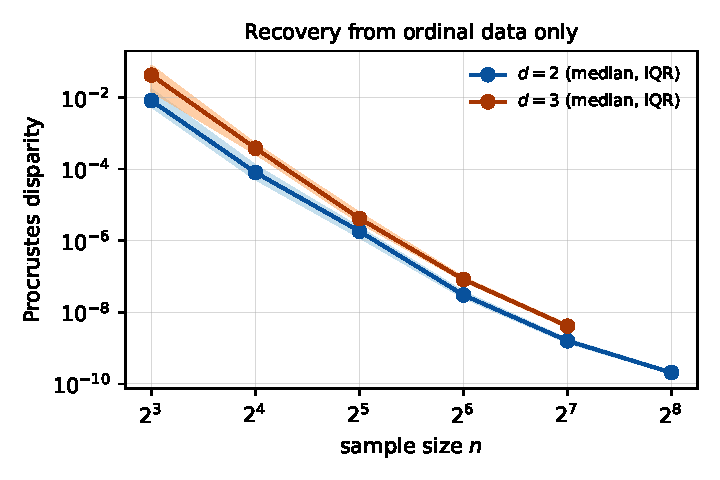
\includegraphics[width=0.62\linewidth]{../figures/ordinal_recovery.pdf}
\caption{E2. Median and interquartile range of the Procrustes disparity of the ordinal reconstruction as a function of $n$, for $d=2$ and $d=3$.}
\label{fig:e2}
\end{figure}

\paragraph{Invariance check (E2b).}
A monotone distortion $D\mapsto D^{p}$, $p\in[2,4]$, leaves the rank matrix literally unchanged, so non-metric scaling, which reads only the rank matrix, returns the identical reconstruction by construction (the reported maximum disparity between the two outputs, \EtwoBordMax{}, is round-off of the alignment); this part of E2b checks the pipeline, not a fact about geometry. The content is in the metric column: metric multidimensional scaling, which uses the values, reconstructs $X$ from $D$ with disparity \EtwoBmetricTrue{} but from $D^p$ with median disparity \EtwoBmetricDist{} (minimum \EtwoBmetricDistMin; $n=\EtwoBn$, \EtwoBreps{} trials). The distortion changes the object of $\Fmet$ and not the object of $\Ford$; this is what ``invariant across formalisms'' means operationally.

\subsection{Measuring the ordinal class directly}

The cautions attached to E2 can be met by measuring the kernel class itself rather than a solver's approximation to it. One measurement is exact.

\begin{proposition}[Thickness of the ordinal class]\label{prop:inradius}
Let $X\in\Fcoord(n,d)$ have distinct pairwise distances and let $g(X)>0$ be the minimal difference between consecutive values in the sorted list of its $m$ pairwise distances. (i)~If $\lVert y_i-x_i\rVert<g(X)/4$ for all $i$, then $Y$ has the same ordinal pattern as $X$. (ii)~If the two pairs of points realising $g(X)$ are disjoint, there is an injective configuration $Y$ with $\max_i\lVert y_i-x_i\rVert=g(X)/4$ in which those two distances coincide (the moved points stay distinct because $g(X)\le\min_{a\ne b}D_{ab}$); $Y$ therefore lies outside the kernel class (its preorder has a tie), and every neighbourhood of $Y$ contains configurations in which the two distances are strictly reversed. Consequently the inradius of the kernel class at $X$, in the norm $\max_i\lVert y_i-x_i\rVert$, lies in $[g(X)/4,\,g(X)/2]$, and equals $g(X)/4$ in case~(ii).
\end{proposition}
\begin{proof}
(i) By the triangle inequality, $\bigl|\lVert y_a-y_b\rVert-\lVert x_a-x_b\rVert\bigr|\le\lVert y_a-x_a\rVert+\lVert y_b-x_b\rVert<g/2$ for every pair, so every distance moves by less than $g/2$ and the difference between any two distances changes by less than $g$; two distances that are consecutive in the sorted order differ by at least $g$ and therefore keep their order, hence so do all pairs. (ii) Let $\{a,b\}$ and $\{c,d\}$ be the disjoint pairs with $D_{cd}-D_{ab}=g$. Move $x_a$ and $x_b$ apart along the line through them by $g/4$ each, and $x_c$ and $x_d$ towards each other along their line by $g/4$ each, leaving the other points fixed: the first distance becomes $D_{ab}+g/2$ and the second $D_{cd}-g/2=D_{ab}+g/2$, a tie, and the four displacements have norm $g/4$. For the upper bound in general, two distinct pairs share at most one point; if $\{a,b\}$ and $\{a,c\}$ realise $g$, moving $x_b$ away from $x_a$ and $x_c$ towards $x_a$ by $g/2$ each produces the same tie. In this shared-point case the smallest displacement that closes the gap depends on the angle $\theta$ at $x_a$: moving $x_a$ as well, in the direction of $e_{ac}-e_{ab}$ ($e_{ab},e_{ac}$ the unit vectors from $x_a$ towards $x_b$ and $x_c$), changes $D_{ab}-D_{ac}$ at first order by $\lVert e_{ab}-e_{ac}\rVert=2\sin(\theta/2)$ per unit of displacement, so the closing displacement is $g/\bigl(2(1+\sin(\theta/2))\bigr)+O(g^2)$; it equals $g/4$ exactly when $x_b,x_a,x_c$ are collinear with $x_a$ between the other two (a configuration the proposition allows), and it approaches $g/2$ as $\theta\to0$. Finally, a configuration outside the class is reached along the segment from $X$ only after two distances that are consecutive at $X$ have tied, so the inradius is the minimum over consecutive pairs of their closing displacements; by (i) no tie occurs below $g/4$, and the constructions above tie the pair realising $g$ at a displacement of at most $g/2$, exactly $g/4$ in case~(ii). The perturbed configurations remain injective, because $g\le\min_{a\ne b}D_{ab}$ for $n\ge3$: if $\{1,2\}$ is the closest pair and $3$ any other point, $|D_{13}-D_{23}|\le D_{12}$ by the triangle inequality, so some consecutive gap is at most $D_{12}$.
\end{proof}

\if\HasClass1
\paragraph{Computational check (E2c).}
For $d=2$ and $n$ from $8$ to $\EtwocNmax$, \EtwocConfigsTotal{} uniform configurations were examined (Table~\ref{tab:e2c}, Figure~\ref{fig:e2c}). Random displacements of every point by a vector of Euclidean norm below $g/4$ preserved the pattern in all \EtwocKeptTotal{} of \EtwocPertTotal{} trials, and the explicit displacement of part~(ii), applied just beyond $g/4$ so that the tie becomes a strict reversal detectable in floating point, changed it in all \EtwocChangedTotal{} of \EtwocChangedTested{} configurations whose extremal pairs were disjoint. The median gap scales as $n^{-\EtwocSlopeGap}$, which is what one expects, heuristically, for the minimal spacing among $m\approx n^2/2$ weakly dependent values with a bounded density, of order $1/m^2\propto n^{-4}$: the class is thin because $n$ points carry $n^2/2$ distances. A second, similarity-invariant measurement is a random walk constrained to the class (proposals accepted only if the ranking is unchanged), which records the largest Procrustes disparity from $X$ among the configurations visited. This \emph{walk range} is a lower bound on the extent of the class at $X$ in that measure, and a loose one: the recorded value grows roughly linearly with the number of steps within the budgets of Table~\ref{tab:e2c} and has not saturated, so neither its value nor its scaling with $n$ ($n^{-\EtwocSlopeWalk}$ for that schedule) measures the class; the scaling is what one expects from an accepted step size proportional to $g$ and a disparity quadratic in the displacement. The walk nevertheless establishes that the class is far wider than its thickness in generic directions: at $n=64$ it stays in the class after displacing every point by several hundred times $g/4$, whereas displacing every point by $g/4$ produces a disparity of order $3g^2/8$ (the squared displacement $n(g/4)^2$ divided by the expected squared centred norm $n/6$ of a uniform sample of the unit square; an order-of-magnitude estimate, not a bound valid for every $X$), that is \EtwocDispEstNsixtyfour{} for the median $g$ at $n=64$, against a walk range of \EtwocWalkNsixtyfour{}. Whether the class extends as far as the residual \EtwoMedDtwoNsixtyfourAgain{} at which the E2 solver stopped (with discordance \EtwoDiscDtwoNsixtyfour) is not decided by these measurements. What the two measurements do establish is the following. No ball of sup-norm radius larger than $g/2$ centred at $X$ fits inside the class, and $g$ decays empirically like $n^{-4}$, so the thickness of the class at a configuration of the unit square shrinks at that rate (Proposition~\ref{prop:inradius} gives thickness in $[g/4,g/2]$, hence exactly at that rate); this bounds the thickness of the class, not its diameter modulo similarity, which is what Theorem~\ref{thm:kvl} controls. An upper bound on that diameter is not established here.

\begin{table}[t]
\centering\footnotesize
\begin{tabular}{rrrrrrr}
\toprule
$n$ & median $g$ & disjoint & kept below $g/4$ & changed beyond $g/4$ & walk steps & median walk range\\
\midrule
8 & \ensuremath{6.7\times 10^{-4}} & 10/20 & 400/400 & 10/10 & 8000 & \ensuremath{5.5\times 10^{-3}} \\
16 & \ensuremath{3.8\times 10^{-5}} & 15/20 & 400/400 & 15/15 & 8000 & \ensuremath{4.4\times 10^{-5}} \\
32 & \ensuremath{4.0\times 10^{-6}} & 16/20 & 400/400 & 16/16 & 6000 & \ensuremath{2.7\times 10^{-7}} \\
64 & \ensuremath{1.9\times 10^{-7}} & 19/20 & 400/400 & 19/19 & 4000 & \ensuremath{1.0\times 10^{-9}} \\
128 & \ensuremath{9.4\times 10^{-9}} & 20/20 & 400/400 & 20/20 & 3000 & \ensuremath{3.8\times 10^{-12}} \\
256 & \ensuremath{6.7\times 10^{-10}} & 11/12 & 240/240 & 11/11 & 1500 & \ensuremath{6.4\times 10^{-15}}
\\
\bottomrule
\end{tabular}
\caption{E2c ($20$ configurations per $n$, $12$ at $n=256$). Median minimal gap $g$ between consecutive sorted distances (the inradius of the class is $g/4$ when the extremal pairs are disjoint), the numerical checks of Proposition~\ref{prop:inradius} (the displacement of part~(ii) is applied with $g/4$ enlarged by $\max(10^{-6}g/4,10^{-12})$ so that the tie becomes a strict reversal), and the median walk range (largest Procrustes disparity from $X$ visited by a random walk confined to the class; a non-saturated lower bound on the extent of the class). Interquartile ranges are shown in Figure~\ref{fig:e2c} and listed in the result files.}
\label{tab:e2c}
\end{table}

\begin{figure}[t]
\centering
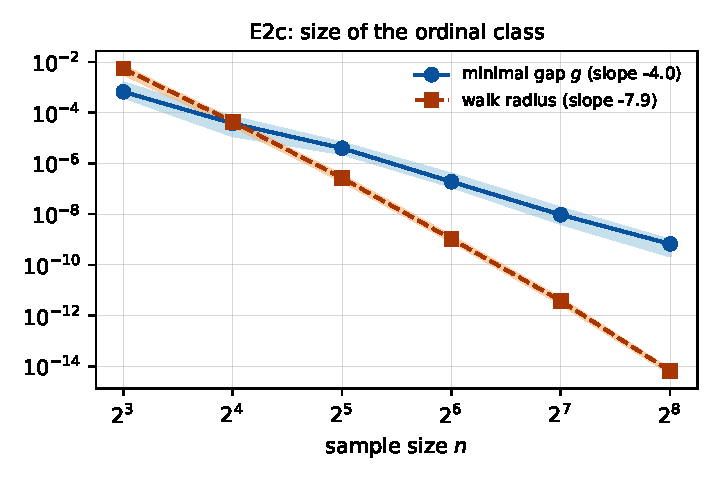
\includegraphics[width=0.62\linewidth]{../figures/ordinal_class.pdf}
\caption{E2c. Median and interquartile range of the minimal gap $g$ and of the walk range against $n$ ($d=2$); the walk range depends on the step budget and is a lower bound only.}
\label{fig:e2c}
\end{figure}
\fi

\section{Formalism depth of geometric quantities}\label{sec:depth}

Lemma~\ref{lem:mono} orders the invariants of the chain, and Section~\ref{sec:euclid} locates the boundaries: position is lost at $\tau_1$, scale at $\tau_2$, everything at $\tau_3$ on generic samples. Table~\ref{tab:e4} classifies familiar quantities by the poorest formalism from which they can be computed, together with a direct computational check (E4): each quantity is computed for $\EfourTrials$ random configurations of $\EfourN$ points in the plane, then recomputed after a random rigid motion, after a random similarity, and after a random monotone distortion $D\mapsto D^p$, $p\in[0.3,3]$, and the fraction of trials in which the value is preserved is reported.

\begin{table}[t]
\centering\small
\begin{tabular}{lcccc}
\toprule
quantity & depth & rigid motion & similarity & monotone distortion\\
\midrule
centroid (position) & coordinate & 0.00 & 0.00 & -- \\
diameter (value) & metric & 1.00 & 0.00 & 0.00 \\
affine dimension & metric & 1.00 & 1.00 & 0.35 \\
Gabriel graph & metric & 1.00 & 1.00 & 0.03 \\
diameter pair & ordinal & 1.00 & 1.00 & 1.00 \\
$k$-nearest-neighbour graph ($k=3$) & ordinal & 1.00 & 1.00 & 1.00 \\
minimum spanning tree & ordinal & 1.00 & 1.00 & 1.00 \\
relative neighbourhood graph & ordinal & 1.00 & 1.00 & 1.00
\\
\bottomrule
\end{tabular}
\caption{E4. Formalism depth of standard quantities and the fraction of \EfourTrials{} trials in which each is preserved under rigid motions (which generate $\ker\tau_1$), similarities, and monotone distortions of the distance matrix (which generate $\ker\tau_2$ on $\Fmet$; the distorted matrix is in general not Euclidean, so this column tests the defining formula on $\Fmet$, a sufficient condition for ordinal depth). The centroid is undefined for a bare metric.}
\label{tab:e4}
\end{table}

The ordinal rows have one-line proofs. The diameter pair is the argument of a maximum, which depends only on the order. The $k$-nearest-neighbour graph is defined by comparisons $D_{ij}<D_{ik}$ within each row. The minimum spanning tree is produced by Kruskal's algorithm from the sorted list of edge weights and is therefore invariant under any strictly monotone reweighting~\citep{kruskal1956}. The relative neighbourhood graph~\citep{toussaint1980} contains $ij$ iff no $k$ satisfies $\max(D_{ik},D_{jk})<D_{ij}$, again a comparison. The metric rows fail for equally simple reasons: the diameter changes under scaling; the affine dimension is the number of positive eigenvalues of the doubly centred squared-distance matrix (Theorem~\ref{thm:classical}), and a power $D^p$ of a planar metric is not planar: for $p<1$ it is a Euclidean metric of dimension at most $n-1$~\citep{schoenberg1937}, for $p>2$ the centred matrix has many positive eigenvalues, and only for $1<p<2$ did it have exactly two positive eigenvalues in every trial, so the value is preserved in a fraction \EfourAffMono{} of trials, essentially the probability that $p\in(1,2)$; the Gabriel graph~\citep{gabriel1969} contains $ij$ iff no $k$ satisfies $D_{ik}^2+D_{jk}^2<D_{ij}^2$, an additive condition, and is preserved in a fraction \EfourGabrielMono{} of trials. That the relative neighbourhood graph is ordinal and the Gabriel graph is not, although both are ``proximity graphs'' of the same family, illustrates that depth is a property of the defining formula, not of the intuitive kind of the quantity. The metric rows are also genuinely non-ordinal on $\Fcoord$, which the distortion column alone does not show, since the distorted matrix leaves the Euclidean locus: a collinear configuration with distinct distances and a small generic perturbation of it share the ordinal pattern (Proposition~\ref{prop:nonunique}) and have affine dimensions $1$ and $2$; a triangle with a right angle at $k$, perturbed to acute or to obtuse without changing the order of its sides, keeps the pattern and gains or loses the Gabriel edge $ij$. Both witnesses are checked in the code (E4b: patterns equal, \EfourbCollinearSame, dimensions \EfourbCollinearDims; patterns equal, \EfourbGabrielSame, edge present \EfourbGabrielEdges).

Theorem~\ref{thm:kvl} adds an asymptotic column to the table: every \emph{continuous} similarity invariant (distance ratios, angles) is asymptotically determined by the ordinal pattern, because the pattern determines the configuration up to similarity in the limit; for discrete invariants such as the Gabriel graph the statement holds only away from configurations near the defining equality, since a dense sample always contains near-borderline pairs. The finite-$n$ classification and the asymptotic one therefore differ, and a claim that ``order determines geometry'' must say which of the two is meant.

\section{A second translation: causal order and counting}\label{sec:lorentz}

The Euclidean chain has an analogue in which the poorer structure is a partial order rather than a ranking. Consider the causal diamond of $1{+}1$ Minkowski space in null coordinates $u=t-x$, $v=t+x$, so that $\dd s^2=\dd u\,\dd v$, the diamond is the unit square $(0,1)^2$, and the proper time between causally related events is $\tau(p,q)=\sqrt{(u_q-u_p)(v_q-v_p)}$. The causal order is the product order, $p\prec q\iff u_p<u_q$ and $v_p<v_q$; unrelated pairs are written $p\incomp q$. The formalisms are:
\begin{itemize}[leftmargin=2em]
\item $\Fcoord_{1,1}(n)$: labelled configurations $(u_i,v_i)_{i\le n}$ in the diamond;
\item $\Fcaus(n)$: partial orders on $[n]$ (labelled); for configurations with pairwise distinct $u$- and pairwise distinct $v$-coordinates (a full-measure open set, assumed throughout), the image of $\sigma_1$ below is the set of labelled orders of Dushnik--Miller dimension at most two~\citep{dushnik1941}, the orders realised by two linear orders, here $<_u$ and $<_v$;
\item $\Fcausn(n)$: the same partial order together with the statistical hypothesis that the configuration is a uniform sample of the diamond, so that counts of points estimate areas; its ``invariants'' are estimators, consistent as $n\to\infty$, rather than functions factoring through a translation.
\end{itemize}
The translation $\sigma_1\colon\Fcoord_{1,1}\to\Fcaus$ forgets the coordinates and keeps the order (the abstract notion of a causal space goes back to \citet{kronheimer1967}); $\Fcausn$ is not a formalism in the sense of Section~\ref{sec:language} but a formalism together with a sampling model, which is what ``number'' means in the causal set slogan. The sequence is therefore a translation followed by a statistical step, not a chain in the sense of Definition~\ref{def:chain}. All statements below are about uniform samples of a fixed background; none is a statement about physics.

\begin{proposition}[Kernel of the order translation]\label{prop:causkernel}
Every map $(u,v)\mapsto(f(u),g(v))$ with $f,g$ strictly increasing bijections of $(0,1)$, and the swap $(u,v)\mapsto(v,u)$, preserve the causal order of every configuration. Boosts $(u,v)\mapsto(\lambda u,v/\lambda)$, as maps of $\R^{1,1}$, preserve the order and in addition all proper times; a general pair $(f,g)$ does not.
\end{proposition}
\begin{proof}
$u_p<u_q\iff f(u_p)<f(u_q)$ for increasing $f$, and likewise for $g$; the swap exchanges the two coordinates in the conjunction defining $\prec$. Under a boost $(\lambda\Delta u)(\Delta v/\lambda)=\Delta u\,\Delta v$. For $f(u)=u^2$, $g=\mathrm{id}$, the proper time between $(0,0)$ and $(u,v)$ becomes $u\sqrt v$.
\end{proof}
The maps $(f,g)$ with $f,g$ increasing homeomorphisms of $(0,1)$ are conformal maps of the diamond onto itself that preserve time and space orientation, and together with the swap (parity) they form a group $(\mathrm{Homeo}^+(0,1))^2\rtimes\mathbb Z_2$ of causal automorphisms of the diamond. The group is infinite-dimensional, which is the well-known reason why Zeeman's theorem, that the causal automorphisms of Minkowski space are generated by the orthochronous Lorentz group, translations and dilations, requires dimension at least three~\citep{zeeman1964}. In the language of Section~\ref{sec:language}, $\ker\sigma_1$ contains the conformal orbits, the analogue of the monotone distortions that generate $\ker\tau_2$ in the Euclidean chain, so $\Inv(\sigma_1)$ is contained in conformal geometry; the inclusion is strict for some configurations at finite $n$ and an equality for others (Proposition~\ref{prop:causnonunique}), and it is always an equality in the continuum theorems: a bijection between past- and future-distinguishing spacetimes that preserves the chronological order in both directions is a smooth conformal isometry~\citep{hawking1976,malament1977}. The finite-sample counterparts are tested next.

\begin{proposition}[Finite non-uniqueness, causal]\label{prop:causnonunique}
Let $n\ge3$ and consider configurations with pairwise distinct $u$- and pairwise distinct $v$-coordinates. The kernel class of such a configuration under $\sigma_1$ is open in $(0,1)^{2n}$, and it is the union of the conformal orbits, modulo the swap, of the realizers $(<_u,<_v)$ of its order. The number of realizers modulo the swap is $1$ for a chain and otherwise equals half the number of transitive orientations of the incomparability graph of the order (the unique realizer $(\prec,\prec)$ of a chain is fixed by the swap, whereas for any other order the reversal of an orientation is a different orientation); it is $n!/2$ for an antichain, and $1$ whenever the incomparability graph has a unique transitive orientation up to reversal (for instance when exactly one pair is unrelated). Hence the kernel class is a single orbit of the group of Proposition~\ref{prop:causkernel} for some configurations and a union of several such orbits for others; both cases occur for every $n\ge3$.
\end{proposition}
\begin{proof}
Under the standing assumption the order is defined by strict inequalities between coordinates, so it is locally constant and the class is open. Two configurations with the same pair of linear orders $(<_u,<_v)$ are related by a pair $(f,g)$ of increasing bijections of $(0,1)$ (interpolate piecewise linearly between the sorted $u$-values of one and of the other, and likewise for $v$), and conversely $(f,g)$ preserves both linear orders while the swap exchanges them; so the conformal orbit modulo the swap of a configuration is exactly the set of configurations with the same realizer modulo the swap, and the kernel class is the union of these sets over the realizers of the order. A realizer is determined by the linear order $<_u$ alone, since $<_v$ is then the reverse of $<_u$ on unrelated pairs and agrees with the order on related ones. Let $T$ be the restriction of $<_u$ to the unrelated pairs; $T$ orients every edge of the incomparability graph, and it is a transitive orientation: if $a\incomp b$, $b\incomp c$ and $a<_u b<_u c$, then $v_a>v_b>v_c$, so $a\incomp c$ and $(a,c)\in T$. Conversely, let $T$ be any transitive orientation of the incomparability graph. Then $\prec\cup T$ is a linear order: it is total and antisymmetric because every pair is either related by $\prec$ or oriented by $T$, and it is transitive because, besides the two pure cases, the mixed case $a\prec b$, $(b,c)\in T$ forces $(a,c)\in\prec\cup T$: the alternatives are $c\prec a$, which gives $c\prec b$ and contradicts $b\incomp c$, and $(c,a)\in T$, which gives $(b,a)\in T$ by transitivity of $T$ and contradicts $a\prec b$; the mirror case $(a,b)\in T$, $b\prec c$ is handled in the same way. Taking $<_u=\prec\cup T$ and $<_v=\prec\cup T^{-1}$ therefore gives a realizer ($<_u\cap<_v=\prec$ because $T$ is antisymmetric), so realizers correspond bijectively to transitive orientations $T$, and reversing $T$ gives the swapped realizer. For a chain the incomparability graph is empty, its only orientation is the empty one and the unique realizer $(\prec,\prec)$ is its own swap, so the count is $1$; for any other order $T\ne T^{-1}$, the orientations pair off and the count is half their number. For an antichain every linear order of $[n]$ is a transitive orientation, giving $n!/2$; when exactly one pair is unrelated the two orientations are reverses of each other. As an explicit example of distinct orbits, three points with $u_2<u_1<u_3$ and $v_3<v_1<v_2$, and three with $u_1<u_2<u_3$ and $v_3<v_2<v_1$, are both antichains and lie in different orbits, since $(f,g)$ preserves the $u$-order and the swap only reverses it.
\end{proof}
The $u$-order is thus a conformal invariant that is not in general an order invariant: what the order alone leaves undetermined at finite $n$ is exactly the choice of a realizer, and the coordinate reconstruction of E5d below makes that choice with the help of the counts. How much is left undetermined for uniform samples is measured in E5e below: for a substantial fraction of samples the realizer is unique, so the order determines the configuration exactly up to the group of Proposition~\ref{prop:causkernel}, and for the rest the ambiguity is a handful of binary choices.

\if\HasLorentz1
\paragraph{Computational check (E5a).}
For \EfiveAtrials{} uniform samples of $n=\EfiveAn$ points, random pairs $(f,g)$ of increasing bijections preserved the order in all \EfiveAconfPreserved{} cases while changing the proper times of related pairs by $\EfiveAconfTauChange\%$ (median over samples of the per-sample median relative change); random boosts preserved the order in all \EfiveAboostPreserved{} cases and the proper times to within a relative $\EfiveAboostTauChange$; a Euclidean rotation of the $(t,x)$ plane by $5^\circ$ to $30^\circ$, which is not a conformal map, changed the relation of a median $\EfiveArotChanged\%$ of the pairs (never fewer than $\EfiveArotChangedMin\%$).

\subsection*{Order alone: dimension}
The fraction of comparable pairs in a uniform sample of a causal diamond is an order invariant with a known expectation in $D$-dimensional Minkowski space, $\Gamma(D+1)\Gamma(D/2)/(2\,\Gamma(3D/2))$, twice the Myrheim--Meyer ratio $\langle R\rangle/N^2$ of ordered relations to ordered pairs, which is the basis of the Myrheim--Meyer dimension estimator~\citep{myrheim1978,meyer1989}. Table~\ref{tab:e5b} reports the observed fractions for $n=\EfiveBn$ points in diamonds of dimension $2$, $3$ and $4$ (\EfiveBreps{} samples each) next to the expected values, and the dimension estimate obtained by inverting the formula. The three dimensions are separated by many standard deviations. This is the Lorentzian analogue of the count of ordinal patterns in Section~\ref{sec:euclid}: a bare order knows the dimension of the space it was sampled from.

\begin{table}[t]
\centering\small
\begin{tabular}{rrrccc}
\toprule
$D$ & $n$ & samples & comparable fraction & expected & dimension estimate\\
\midrule
2 & 400 & 60 & $0.4989 \pm 0.0185$ & 0.5000 & $2.00 \pm 0.05$ \\
3 & 400 & 60 & $0.2298 \pm 0.0167$ & 0.2286 & $3.00 \pm 0.09$ \\
4 & 400 & 60 & $0.1005 \pm 0.0121$ & 0.1000 & $4.00 \pm 0.14$
\\
\bottomrule
\end{tabular}
\caption{E5b. Fraction of comparable pairs (mean $\pm$ sd over samples) in uniform samples of causal diamonds of Minkowski space of dimension $D$, the expected value, and the Myrheim--Meyer estimate of $D$.}
\label{tab:e5b}
\end{table}

\subsection*{Order plus number: proper time}
For related points $p\prec q$ let $L(p,q)$ be the number of links of the longest chain from $p$ to $q$, an order invariant. In the $1{+}1$ diamond a chain is an increasing sequence in both coordinates, so $L(p,q)-1$ is the length of the longest increasing subsequence of the points inside the rectangle spanned by $p$ and $q$, whose expected number is $N=(n-2)\,\tau(p,q)^2$. Uniform points in a rectangle induce a uniformly random permutation, so by the Vershik--Kerov and Logan--Shepp theorem the longest increasing subsequence of $N$ of them has length $2\sqrt N\,(1+o(1))$~\citep{vershik1977,loganshepp1977}; \citet{brightwell1991} and \citet{bollobas1991} give the corresponding statements for sprinklings in Minkowski space of any dimension, and \citet{bollobas1992} the concentration of the chain length. Hence
\[
L(p,q)\;\approx\;2\sqrt n\;\tau(p,q),
\]
and $\hat\tau=L/(2\sqrt n)$ estimates the proper time from the order and the density alone. Table~\ref{tab:e5c} reports, for $n$ from $\EfiveCnmin$ to $\EfiveCnmax$ and \EfiveCpairsTotal{} related pairs in total, the correlation between $L$ and $\tau$, the least-squares slope through the origin of $L$ against $\sqrt n\,\tau$, and the median relative error of $\hat\tau$. At $n=\EfiveCnmax$ the correlation is \EfiveCcorrLast{} and the slope \EfiveCslopeLast{} (it is \EfiveCslopeFirst{} at $n=\EfiveCnmin$; the mean length of the longest increasing subsequence is $2\sqrt N$ minus a correction of order $N^{1/6}$ with a negative constant~\citep{baik1999}, which is why all slopes lie below $2$); the median relative error of $\hat\tau$ over pairs with $\tau>1/4$ falls from $\EfiveCerrFirst\%$ to $\EfiveCerrLast\%$. The same table shows what ``number'' contributes: after a random conformal reparametrisation $(f,g)$ the order, and hence $L$, is unchanged (this is asserted in the code for every pair), but the same $\hat\tau$ misses the proper times $\tau'$ of the reparametrised configuration by a median of $\EfiveCerrDistLast\%$ at $n=\EfiveCnmax$ (and their correlation with $L$ drops to \EfiveCcorrDistLast); given E5a this is expected rather than independent evidence, and it is reported as an illustration. The chain length estimates the proper time of the frame in which the sample is uniform: the counting measure selects the conformal factor, and without it the order alone cannot.

\begin{table}[t]
\centering\small
\begin{tabular}{rrccccc}
\toprule
$n$ & pairs & corr$(L,\tau)$ & corr$(L,\tau')$ & slope & rel.\ err.\ vs $\tau$ & rel.\ err.\ vs $\tau'$\\
\midrule
250 & 12000 & 0.967 & 0.856 & 1.732 & 0.143 & 0.229 \\
500 & 12000 & 0.978 & 0.866 & 1.739 & 0.138 & 0.217 \\
1000 & 9000 & 0.988 & 0.871 & 1.792 & 0.104 & 0.217 \\
2000 & 6000 & 0.990 & 0.909 & 1.854 & 0.082 & 0.166
\\
\bottomrule
\end{tabular}
\caption{E5c. Longest-chain length $L$ against proper time $\tau$ in uniform samples of the $1{+}1$ diamond; $\tau'$ is the proper time after a random conformal reparametrisation, under which $L$ is unchanged. Slope: least-squares coefficient through the origin of $L$ on $\sqrt n\,\tau$ (limit $2$). Last two columns: median relative error of $\hat\tau=L/(2\sqrt n)$ against $\tau$ and against $\tau'$, over pairs with $\tau>\tfrac14$.}
\label{tab:e5c}
\end{table}

\subsection*{Order plus number: coordinates}
Under uniform density, $|{\downarrow}q|\approx (n-1)\,u_qv_q$ and $|{\uparrow}q|\approx(n-1)(1-u_q)(1-v_q)$ for the past and future of $q$, so the order and the count give $s=u_q+v_q$ and $p=u_qv_q$ and hence the unordered pair $\{u_q,v_q\}$ as the roots of $x^2-sx+p$. Which root is $u_q$ is a sign per point. Both kinds of pairs constrain the relative signs: a comparable pair must satisfy $(u_r-u_q)(v_r-v_q)>0$ and an unrelated pair $r\incomp q$ must satisfy $(u_r-u_q)(v_r-v_q)<0$, and whenever exactly one of the two relative orientations satisfies the constraint the pair votes ``same'' or ``opposite'' (an ablation that uses the votes of unrelated pairs only changes the median error at $n=\EfiveDnmax$ by \EfiveDablation{}, from \EfiveDrmseLastFour{} to \EfiveDrmseAblLastFour{}); the votes are resolved globally by the leading eigenvector of the vote matrix, and the remaining global swap is the parity of Proposition~\ref{prop:causkernel}, which no order can fix. The result is a reconstruction of every coordinate, not merely of the configuration up to a group, because the boundary of the diamond is part of the sampling hypothesis. Table~\ref{tab:e5d} reports the root-mean-square coordinate error over $n$ from $\EfiveDnmin$ to $\EfiveDnmax$: the median falls from \EfiveDrmseFirst{} to \EfiveDrmseLast{}, roughly as $n^{-\EfiveDexponent}$ over the range, slower than the $n^{-1/2}$ fluctuation of the counts; the loss is expected from the ill-conditioning of the roots near $u=v$, where the discriminant $s^2-4p$ vanishes and an $O(n^{-1/2})$ error in the counts becomes an $O(n^{-1/4})$ error in the roots (the rate is not established here). The order recomputed from the reconstructed coordinates disagrees with the true order on $\EfiveDdisagreeLast\%$ of the pairs at $n=\EfiveDnmax$. Figure~\ref{fig:e5} shows one instance.

\begin{table}[t]
\centering\small
\begin{tabular}{rrrrrr}
\toprule
$n$ & samples & median RMSE & max RMSE & median RMSE $\times\sqrt n$ & order disagreement\\
\midrule
250 & 10 & 0.0732 & 0.0971 & 1.16 & 7.62\% \\
500 & 10 & 0.0494 & 0.0622 & 1.10 & 5.24\% \\
1000 & 6 & 0.0415 & 0.0544 & 1.31 & 4.53\% \\
2000 & 4 & 0.0312 & 0.0379 & 1.39 & 3.68\%
\\
\bottomrule
\end{tabular}
\caption{E5d. Root-mean-square error of the coordinates $(u,v)$ recovered from the causal order and the past/future counts (after fixing the global swap), and the fraction of pairs whose comparability differs between the true and the reconstructed configuration.}
\label{tab:e5d}
\end{table}

\begin{figure}[tb]
\centering
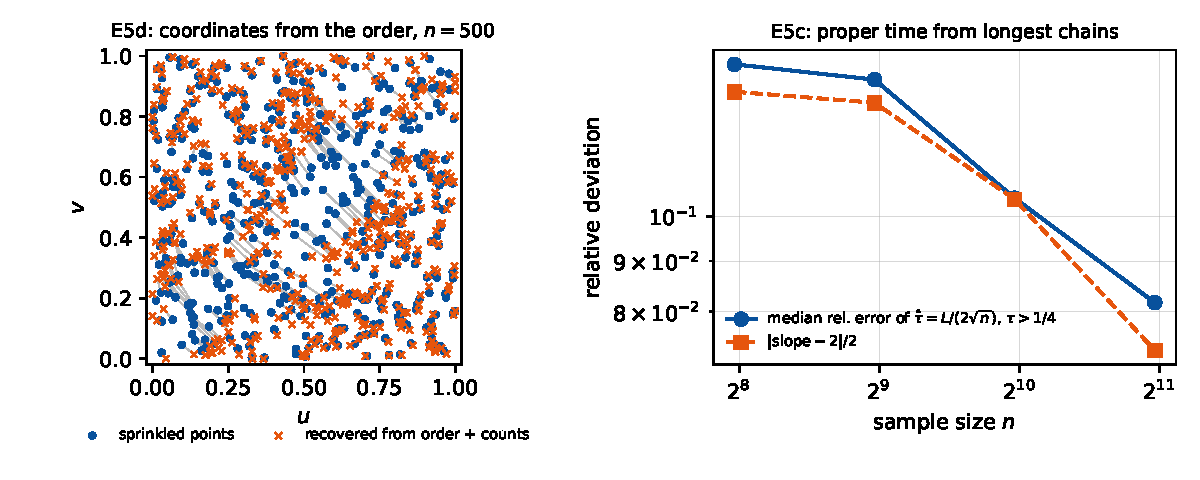
\includegraphics[width=0.9\linewidth]{../figures/lorentz_chain.pdf}
\caption{Left (E5d): a uniform sample of the $1{+}1$ diamond and the coordinates recovered from its causal order and counts. Right (E5c): relative error of the chain-length estimate of proper time and relative deviation of the fitted slope from $2$, against $n$.}
\label{fig:e5}
\end{figure}

\subsection*{Order alone: how many realizers?}
Proposition~\ref{prop:causnonunique} reduces the finite-$n$ ambiguity of the order to the count of its realizers modulo the swap. E5e computes this count for uniform samples by enumerating the transitive orientations of the incomparability graph over its implication colour classes (Golumbic's $\Gamma$-relation~\citep{golumbic1977,golumbic1980}; every transitive orientation contains each implication class or its reverse, so the $2^k$ choices over the $k$ classes exhaust the candidates) and checking transitivity, cross-checked against a brute-force enumeration of pairs of linear extensions at $n=6$ (\EfiveEcrossAgree{} of \EfiveEcrossTested{} agree). Table~\ref{tab:e5e} shows that the realizer is unique for a fraction \EfiveEuniqueNmax{} of the samples at $n=\EfiveEnmax$, and that at most eight realizers occur in a fraction \EfiveEleEightNmax{}: for those samples the causal order determines the configuration exactly up to the group of Proposition~\ref{prop:causkernel}, or up to a few binary choices. The extra realizers typically come from pairs of points that are adjacent in both coordinate orders with opposite directions. Such a pair consists of incomparable twins (every other point relates to both in the same way) and is therefore a module of the incomparability graph, which a transitive orientation can orient in two ways independently of the rest; in the typical situation for large $n$, made precise below, these pairs are the only modules that affect the count, and Lemma~\ref{lem:inflation} with Theorem~\ref{thm:gallai} gives $2\cdot2^N$ transitive orientations, hence $2^N$ realizers modulo the swap, where $N$ is the number of such pairs. $N$ is the number of descending successions of the permutation that sends $u$-ranks to $v$-ranks; it has mean $(n-1)/n$ and is asymptotically Poisson with mean one, a classical result on runs of consecutive elements in random permutations~\citep{wolfowitz1944,kaplansky1945} (Theorem~\ref{thm:realizers}(b) below gives its factorial moments exactly). These pairs are not the only source of ambiguity (at $n=10$ the largest count observed is \EfiveEmaxCountNten, which is not a power of two and comes from larger modules of mutually unrelated points), but the other sources become rare as $n$ grows. Version~0.5 of this draft stated the resulting law as a conjecture; it is proved next.

\paragraph{The realizer law.}
Sort the points of a configuration by $u$ and let $\pi(i)$ be the $v$-rank of the $i$-th point. For independent uniform points $u$ and $v$ are independent and continuous, so $\pi$ is uniform on the symmetric group $S_n$, and the $i$-th point precedes the $j$-th iff $i<j$ and $\pi(i)<\pi(j)$. The unrelated pairs are the inversions of $\pi$, so the incomparability graph of the order is the permutation graph $G_\pi$ of $\pi$ (vertices $1,\dots,n$, an edge $ij$ iff $(i-j)(\pi(i)-\pi(j))<0$), and by Proposition~\ref{prop:causnonunique} the number of realizers modulo the swap is $R(\pi)=1$ if $\pi$ is the identity and $R(\pi)=t(G_\pi)/2$ otherwise, where $t(G)$ is the number of transitive orientations of $G$. A pair of points adjacent in both coordinate orders with opposite directions is an index $i$ with $\pi(i+1)=\pi(i)-1$ (a \emph{descending succession}); $N(\pi)$ denotes their number. An \emph{interval} of $\pi$ is a set of consecutive positions whose values are consecutive integers; it is trivial if it has $1$ or $n$ elements, and $\pi$ is \emph{simple} if all its intervals are trivial. A \emph{module} of a graph is a set $M$ of vertices such that every vertex outside $M$ is adjacent to all or to none of $M$; it is trivial if $|M|\le1$ or $M$ is the whole vertex set, and the graph is \emph{prime} if all its modules are trivial. For $\sigma\in S_m$ and permutations $\alpha_1,\dots,\alpha_m$, the inflation $\sigma[\alpha_1,\dots,\alpha_m]$ replaces the $j$-th entry of $\sigma$ by a block of consecutive positions with consecutive values in the pattern $\alpha_j$, the blocks being ordered by value as the entries of $\sigma$. We use one result from the theory of comparability graphs that is not proved here.

\begin{theorem}[Gallai~\citep{gallai1967}]\label{thm:gallai}
A prime comparability graph with at least three vertices has exactly two transitive orientations, one the reverse of the other. \status{literature}
\end{theorem}

\noindent The restriction to at least three vertices excludes the two-vertex graph without edges, which is prime in the sense above and has only the empty orientation. Permutation graphs are comparability graphs ($G_\pi$ is the comparability graph of the order $i<j$, $\pi(i)>\pi(j)$), so Theorem~\ref{thm:gallai} applies to them\if\HasRlawChk1; it was also checked numerically on all \RlawChkGallaiSimple{} simple permutations of length $4$ to \RlawChkGallaiNmax{} (Appendix~\ref{app:realizers})\fi. In a transitive orientation we write $x\to y$; the basic forcing rule~\citep{gallai1967,golumbic1980} is that if $x$ is adjacent to $a$ and $b$ and $a$, $b$ are not adjacent, then $x\to a$ iff $x\to b$, since $a\to x\to b$, like $b\to x\to a$, would force the edge $ab$ by transitivity. Not every module of $G_\pi$ is an interval of $\pi$ (for the identity, $G_\pi$ has no edges and $\{1,3\}$ is a module), but the two notions agree where it matters.

\begin{lemma}[Intervals and modules]\label{lem:simpleprime}
Every interval of $\pi$ is a module of $G_\pi$. Conversely, if $n\ge3$ and $G_\pi$ has a module $M$ with $2\le|M|\le n-1$, then $\pi$ has an interval with between $2$ and $n-1$ elements. Hence, for $n\ge3$, $\pi$ is simple iff $G_\pi$ is prime, and no permutation of length $3$ is simple. \status{known, e.g.~\citep{brignall2010}; proof included for completeness}
\end{lemma}

\begin{lemma}[Inflation of a simple permutation]\label{lem:inflation}
If $\sigma\in S_m$ is simple, $m\ge4$, and $\pi=\sigma[\alpha_1,\dots,\alpha_m]$, then $t(G_\pi)=2\prod_{j=1}^m t(G_{\alpha_j})$. \status{classical, the prime-node case of Gallai's decomposition~\citep{gallai1967}; proof included for completeness}
\end{lemma}

\begin{theorem}[Realizer law]\label{thm:realizers}
Let $R_n$ be the number of realizers modulo the swap of the causal order of $n$ independent uniform points of the $1{+}1$ diamond, and $N_n$ the number of pairs of points adjacent in both coordinate orders with opposite directions. For $n\ge20$:
\begin{enumerate}[label=(\alph*),leftmargin=2em]
\item $\Pr(R_n\ne2^{N_n})\le 10/n+166/n^2$;
\item $\mathbb E[N_n(N_n-1)\cdots(N_n-r+1)]=1-r/n$ for $0\le r\le n-1$; hence $N_n\to Z\sim\mathrm{Po}(1)$ in law.
\end{enumerate}
\status{proved here, using Theorem~\ref{thm:gallai}}
\end{theorem}

\noindent Consequently $R_n\to2^Z$ in law. Theorem~\ref{thm:sharpN} and Proposition~\ref{prop:sharpexplicit} below give the rate $O(1/n)$ with explicit constants; in particular the fractions of samples with one, two and at most eight realizers tend to $e^{-1}$, $e^{-1}$ and $\tfrac83e^{-1}$, each with error $O(1/n)$.

\begin{proposition}[Where the exceptions come from]\label{prop:exceptions}
$\Pr(R_n\ne2^{N_n})=3(n-2)/(n(n-1))+2/n+O(n^{-2})=5/n+O(n^{-2})$. Up to an event of probability $O(n^{-2})$, an exception is a configuration with a single interval of three elements in one of the patterns $321$ (then $R_n=\tfrac32\,2^{N_n}$), $231$ or $312$ (then $R_n=2\cdot2^{N_n}$), or with $\pi(1)=n$ or $\pi(n)=1$, i.e.\ a point related to no other one and extreme in both coordinate orders (then $R_n=2\cdot2^{N_n}$). \status{proved here, using Theorem~\ref{thm:gallai}}
\end{proposition}

\paragraph{Sharp rates.}
Theorem~\ref{thm:realizers} gives no rate for $N_n$, and its bound~(a) is about twice the true rate; the exact first-order terms are as follows. Write $p_k=\Pr(N_n=k)$ and $q_k=e^{-1}/k!$ for $k\ge0$, $q_k=0$ for $k<0$, and $Z\sim\mathrm{Po}(1)$. The three results below were added in version~0.7; they are proved in Appendix~\ref{app:realizers} and checked numerically there, and they were checked by an independent internal referee in round~5 (step by step, and by exhaustive enumeration of $S_n$ for $n\le11$).

\begin{theorem}[Sharp Poisson rate for $N_n$]\label{thm:sharpN}
\begin{enumerate}[label=(\roman*),leftmargin=2em]
\item For $n\ge1$ and $0\le k\le n-1$,
\[
p_k=q_k\Bigl(1-\frac{k-1}{n}\Bigr)+r_{n,k},\qquad |r_{n,k}|\le\frac{1}{n\,k!\,(n-k+1)!}.
\]
Equivalently $p_k=q_k+\nu(k)/n+r_{n,k}$ with $\nu(k)=q_k-q_{k-1}=-(k-1)q_k$; for fixed $k$ the remainder is smaller than any power of $n$.
\item For $n\ge4$, $d_{\mathrm{TV}}(N_n,\mathrm{Po}(1))=(p_0-q_0)+(p_1-q_1)^+$, and
\[
\Bigl|\,d_{\mathrm{TV}}(N_n,\mathrm{Po}(1))-\frac{e^{-1}}{n}\Bigr|<\frac{2}{n\cdot n!}.
\]
Hence $n\,d_{\mathrm{TV}}(N_n,\mathrm{Po}(1))\to c_1=\tfrac{e^{-1}}2\sum_{k\ge0}|k-1|/k!=e^{-1}$. (The identity and the bound also hold for $n\le3$, by direct computation; $n\ge4$ is used only in the proof.)
\end{enumerate}
\status{proved here, an elementary consequence of the classical exact law~\citep{kaplansky1945}; checked by an independent internal referee (round~5)}
\end{theorem}

\begin{theorem}[First-order law of the realizer count]\label{thm:sharpR}
Let $\mu$ be the signed measure on $\{2^k\}_{k\ge0}\cup\{3\cdot2^k\}_{k\ge1}$ given by
\[
\mu(\{2^k\})=-3q_k+3q_{k-1}-q_{k-2}=-\frac{e^{-1}}{k!}(k-1)(k-3),\qquad
\mu(\{3\cdot2^k\})=q_{k-1}=\frac{e^{-1}}{(k-1)!}.
\]
Then $\mu$ has total mass $0$, and uniformly over sets $A$ of positive reals,
\[
\Pr(R_n\in A)=\Pr(2^Z\in A)+\frac{\mu(A)}{n}+O(n^{-2}).
\]
Consequently
\[
d_{\mathrm{TV}}(R_n,2^Z)=\frac{c_2}{n}+O(n^{-2}),\qquad c_2=\tfrac12\lVert\mu\rVert=1+\frac1{2e}=\SharpCtwoLong\ldots
\]
In particular, with errors $O(n^{-2})$: $\Pr(R_n=1)=e^{-1}(1-3/n)$, $\Pr(R_n=2)=e^{-1}$, $\Pr(R_n=4)=\tfrac12e^{-1}(1+1/n)$, $\Pr(R_n=6)=\Pr(R_n=12)=e^{-1}/n$, $\Pr(R_n\le8)=\tfrac83e^{-1}-\tfrac32e^{-1}/n$, and $\Pr(R_n\text{ is not a power of }2)=1/n$. \status{proved here, using Theorem~\ref{thm:gallai}; checked by an independent internal referee (round~5)}
\end{theorem}

\begin{proposition}[Explicit bounds]\label{prop:sharpexplicit}
For $n\ge20$,
\[
\Pr(R_n\ne2^{N_n})\le\frac5n+\frac{220}{n^2},\qquad
d_{\mathrm{TV}}(R_n,2^Z)\le\frac{5+e^{-1}}{n}+\frac{221}{n^2}.
\]
\status{proved here, using Theorem~\ref{thm:gallai}; checked by an independent internal referee (round~5)}
\end{proposition}

\noindent The measure $\mu$ is the sum of three contributions: the first-order term $\nu$ of the law of $N_n$ (a mean shift, $\mathbb E N_n=1-1/n$); the configurations with a three-element interval of pattern $321$, which have probability $1/n+O(n^{-2})$ and $R_n=6\cdot2^{N_n-2}$; and the four configurations with $R_n=2\cdot2^{N_n}$ (patterns $231$, $312$, $\pi(1)=n$, $\pi(n)=1$), of total probability $4/n+O(n^{-2})$. The latter move mass from $2^{j}$ to $2^{j+1}$, atoms that $2^Z$ charges anyway, so they largely cancel in the total variation distance: the coupling bound $\Pr(R_n\ne2^{N_n})+d_{\mathrm{TV}}(N_n,Z)$ has first-order constant $5+e^{-1}$, the true one is $1+1/(2e)$. The positive part of $\mu$ consists of the atoms $3\cdot2^k$ (mass $1$) and the atom $4$ (mass $e^{-1}/2$).

\paragraph{Second order.}
The results below were added in version~0.8; they are proved in Appendix~\ref{app:realizers} and checked numerically there, but have not yet been checked by an independent referee. For $\lambda>0$ write $q_k(\lambda)=e^{-\lambda}\lambda^k/k!$, so that $q_k=q_k(1)$, and $\tilde q_k=q_k(1-1/n)$; for integers $j,k\ge0$ let $c_j(k)=\sum_{i=0}^{j}(-1)^i\binom ki/(j-i)!$ be the coefficient of $x^j$ in $e^x(1-x)^k$, so that $c_0=1$, $c_1(k)=1-k$, $c_2(k)=\tfrac12(k^2-3k+1)$ and $\tilde q_k=q_k\sum_{j\ge0}c_j(k)n^{-j}$. The remainder $r_{n,k}$ is that of Theorem~\ref{thm:sharpN}(i).

\begin{theorem}[Second-order law of $N_n$]\label{thm:secondN}
\begin{enumerate}[label=(\roman*),leftmargin=2em]
\item For $n\ge1$ and $0\le r\le n-1$, $\mathbb E[(N_n)_r]-(1-1/n)^r=-\binom r2n^{-2}+\theta\binom r3n^{-3}$ with $\theta\in[0,1]$, where $(N)_r=N(N-1)\cdots(N-r+1)$; and for $0\le k\le n-1$,
\[
p_k=\tilde q_k-q_k\sum_{j\ge2}\frac{c_j(k)}{n^{j}}+r_{n,k}=\tilde q_k-q_k\,\frac{k^2-3k+1}{2n^2}+O_k(n^{-3}).
\]
\item For $n\ge3$,
\[
d_{\mathrm{TV}}\bigl(N_n,\mathrm{Po}(1-1/n)\bigr)=\Phi(1/n)+\varepsilon_n,\qquad
|\varepsilon_n|\le\frac{2^{n+1}-n-2}{n\,(n+1)!},
\]
where $\Phi(x)=\tfrac12e^{-1}(3-x)\bigl(1-(1-x)e^{x}\bigr)$.
\item For $n\ge3$, $0<n^2\Phi(1/n)-\frac3{4e}-\frac1{4en}\le\frac1{48en^2}$. Hence
\[
n^2d_{\mathrm{TV}}\bigl(N_n,\mathrm{Po}(1-1/n)\bigr)=\frac3{4e}+\frac1{4en}+O(n^{-2})\longrightarrow\frac3{4e}=\SecThreeFourE\ldots
\]
\end{enumerate}
\status{proved here; not yet independently refereed}
\end{theorem}

\noindent The first-order measure $q+\nu/n$ of Theorem~\ref{thm:sharpN} has factorial moments exactly $1-r/n$ for every $r$ (since $\sum_k\nu(k)(k)_r=1-\mathbb E[(Z+1)_r]=-r$), consistent with its super-exponentially small distance to the law of $N_n$; $\mathrm{Po}(1-1/n)$ matches the mean but not the second factorial moment, and the mismatch $-\binom r2/n^2$ is the term $-q_kc_2(k)/n^2$ of~(i). Since $\sum_kq_kc_2(k)=0$ and $c_2(k)<0$ only for $k=1,2$, $\tfrac12\sum_kq_k|c_2(k)|=\tfrac3{4e}$, the constant of~(iii); version~0.7 reported this limit only numerically. The mean-matching Poisson law is not the closest one at this order.

\begin{theorem}[Best Poisson approximation of $N_n$]\label{thm:bestpois}
For real $a$ let $L(a)=\sum_{k\ge0}q_k\,|c_2(k)+a(k-1)|$.
\begin{enumerate}[label=(\roman*),leftmargin=2em]
\item For every fixed $a$, $n^2d_{\mathrm{TV}}(N_n,\mathrm{Po}(1-1/n+a/n^2))\to L(a)/2$.
\item $L(a)\ge e^{-1}$, with equality if and only if $a=\tfrac12$; for $a\ge-\tfrac14$, $L(a)=e^{-1}\bigl(1+(2a-1)^++(\tfrac12-a)^+\bigr)$, so $L(0)/2=3/(4e)$.
\item $n^2\inf_{\lambda>0}d_{\mathrm{TV}}(N_n,\mathrm{Po}(\lambda))\to1/(2e)=\SecOneTwoE\ldots$, and $\lambda_n=1-1/n+1/(2n^2)$ attains this limit.
\end{enumerate}
\status{proved here; not yet independently refereed}
\end{theorem}

\begin{proposition}[Explicit constant in Theorem~\ref{thm:sharpR}]\label{prop:sharpC}
For every $n\ge22$ and every set $A$ of positive reals, $|\Pr(R_n\in A)-\Pr(2^Z\in A)-\mu(A)/n|\le B(n)$, where $B(n)$ is the explicit function~\eqref{eq:Bn} of Appendix~\ref{app:realizers}, and $n^2B(n)$ is non-increasing. Consequently
\[
\Bigl|d_{\mathrm{TV}}(R_n,2^Z)-\frac{c_2}{n}\Bigr|\le\frac{\SecCtwentytwo}{n^2}\quad(n\ge22),\qquad\le\frac{\SecChundred}{n^2}\quad(n\ge100),
\]
and $n^2B(n)\to259+10/e=\SecClimit\ldots$ \status{proved here, using Theorem~\ref{thm:gallai}; not yet independently refereed}
\end{proposition}

\noindent The constant is far from sharp: from the exact law of $R_n$ for $n\le\SecFloatNmax$ (Appendix~\ref{app:realizers}), $n^2|d_{\mathrm{TV}}(R_n,2^Z)-c_2/n|$ is at most \SecDtvMaxTT{} for $22\le n\le\SecFloatNmax$ and at most \SecDtvMaxAll{} for $4\le n\le\SecFloatNmax$. Most of the gap comes from the bad event $\mathcal E$ of Lemma~\ref{lem:sharpbad} and the occurrences inside it, which the proof charges in full ($90+150$ of the limit $259+10/e$).

\begin{remark}[What remains open]\label{rem:secondopen}
The $n^{-2}$ term of the law of $R_n$ is not proved. Numerically (exact laws for $n\le\SecFloatNmax$, polynomial fits in $1/n$ on $\SecFitLo\le n\le\SecFitHi$), $n^2\bigl(\Pr(R_n=x)-\Pr(2^Z=x)-\mu(x)/n\bigr)$ converges for each of the \SecAtomsN{} atoms $x\in\{2^k,3\cdot2^k\}$ with $k<\SecAtomsK$, $n^2\Pr(R_n\notin\{2^k,3\cdot2^k\}_{k\ge0})$ approaches \SecUntracked, and
\[
n^2\Bigl(d_{\mathrm{TV}}(R_n,2^Z)-\frac{c_2}n\Bigr)\to\kappa\approx\SecKappa,
\]
the fits of degree $2$, $3$ and $4$ giving \SecKappaTwo, \SecKappaThree{} and \SecKappaFour. \status{open; $\kappa$ computationally verified (extrapolation of exact values), not proved}
\end{remark}

\begin{conjecture}[Closed form of the second-order term]\label{conj:kappa}
Let $\mu_2(x)=\lim_n n^2\bigl(\Pr(R_n=x)-\Pr(2^Z=x)-\mu(x)/n\bigr)$. Then $\mu_2(2^k)=q_k\bigl[12\binom k4-12\binom k3+12\binom k2-3k-5\bigr]$, $\mu_2(3\cdot2^k)=(k+1)q_{k-1}$ for $k\ge1$, and $\mu_2(3)=0$; with the mass $\tfrac12$ outside these atoms this gives $\kappa=\mu_2(4)+\mu_2(8)+\sum_{k\ge1}\mu_2(3\cdot2^k)+\tfrac12=\tfrac72+\tfrac{13}{6e}=\SecKappaConj\ldots$ \status{conjectural: read off the numbers, which agree with these forms within \SecMuTwoDev{} at the \SecAtomsN{} atoms of Remark~\ref{rem:secondopen}}
\end{conjecture}

\paragraph{Outline of the proofs.}
The complete proofs are in Appendix~\ref{app:realizers}. Lemma~\ref{lem:simpleprime} is the usual correspondence between intervals and modules, and Lemma~\ref{lem:inflation} is the prime-node case of Gallai's decomposition: the blocks are modules, the quotient is prime, and a transitive orientation is one of the two of the quotient together with independent ones of the blocks. Theorem~\ref{thm:realizers} combines them with a first-moment bound on intervals and an exact inclusion--exclusion for successions: if $\pi$ has no interval with between $3$ and $n-1$ elements, contracting its successions, which are disjoint, gives a simple permutation of length at least $4$, and $R_n=2^{N_n}$; the expected number of intervals with $k$ elements is $(n-k+1)^2k!\,(n-k)!/n!$, that is $6/n+O(n^{-2})$ for $k=3$, $4/n$ for $k=n-1$ and $O(n^{-2})$ in total for the other $k$. This first-moment computation is classical: the number of non-trivial intervals of a uniform permutation converges to a Poisson law of mean $2$~\citep{corteel2006}, and a uniform permutation is simple with probability $e^{-2}(1-4/n+O(n^{-2}))$~\citep{albert2003}. What we have not found in the literature, and claim as new, is the assembly of these facts in the causal translation, the explicit constants, and the classification of the exceptions in Proposition~\ref{prop:exceptions}: up to probability $O(n^{-2})$ there is at most one interval with between $3$ and $n-1$ elements, it has $3$ or $n-1$ elements, and its pattern, or the extreme point it leaves out, multiplies the count by $\tfrac32$ or $2$. Theorem~\ref{thm:sharpN} evaluates the alternating tail of the exact inclusion--exclusion of Step~3; Theorem~\ref{thm:sharpR} conditions on the single exceptional configuration of Proposition~\ref{prop:exceptions}, contracts it, and bounds the event with two or more configurations by second moments. Theorems~\ref{thm:secondN} and~\ref{thm:bestpois} compare the exact law of $N_n$ with Poisson laws through the signs of $e^x(1-x)^k-1-(1-k)x$, and Proposition~\ref{prop:sharpC} bounds each error term of the proof of Theorem~\ref{thm:sharpR}.

\paragraph{Sharpness and data.}
The bound in Theorem~\ref{thm:realizers}(a) counts every interval and is about twice the true rate $5/n$ of Proposition~\ref{prop:exceptions}; by Theorem~\ref{thm:sharpN}, $d_{\mathrm{TV}}(N_n,\mathrm{Po}(1))$ equals $e^{-1}/n$ up to $2/(n\cdot n!)$\if\HasRlawChk1, which is why the numerical value $n\,d_{\mathrm{TV}}(N_n,\mathrm{Po}(1))=\RlawChkNdTV$ was found at every $n$ tested (Appendix~\ref{app:realizers})\fi. \if\HasRlaw1 The limits \RlawPoissonOne, \RlawPoissonOne{} and \RlawPoissonLeThree{} are consistent with Table~\ref{tab:e5e}, where the three fractions at $n=\EfiveEnmax$ are \EfiveEuniqueNmax, \EfiveEtwoNmax{} and \EfiveEleEightNmax, and with the independent samples of E5f (Table~\ref{tab:e5f}): the exact count equalled $2^N$ in a fraction \RlawEqualFracNmin{} of the samples at $n=\RlawNmin$, in \RlawEqualBig{} of the \RlawSamplesBig{} samples with $n\ge\RlawBigNmin$, and in \RlawEqualNmax{} of \RlawSamplesNmax{} at $n=\RlawNmax$; these samples are too small to resolve the $1/n$ terms\if\HasSharp1, which the larger samples of Table~\ref{tab:sharp} do\fi. The ratios $R/2^N$ among the exceptions are \RlawRatiosAll{} over all $n$, but only \RlawRatiosBig{} for $n\ge\RlawBigNmin$, as Proposition~\ref{prop:exceptions} predicts; the larger ratios come from events of probability $O(n^{-2})$ (Remark~\ref{rem:exact}). \fi\if\HasRlawChk1 With larger samples of uniform permutations (\RlawChkSamplesMin{} to \RlawChkSamplesMax{} per $n$, Appendix~\ref{app:realizers}), $n\Pr(R_n\ne2^{N_n})$ lies between \RlawChkNPlo{} and \RlawChkNPhi{} for $n$ from \RlawChkNlo{} to \RlawChkNhi; \RlawChkCIcontainFive{} of its \RlawChkCIrows{} confidence intervals at level $95\%$ contain $5$, and they widen from \RlawChkCIfirst{} at $n=\RlawChkNlo$, where the agreement is partly fortuitous because the event of probability $O(n^{-2})$ is not small\if\HasSharp1{} (it accounts for \SharpFTwentyExcBad{} of \SharpFTwentyExc{} exceptions at $n=20$, Appendix~\ref{app:realizers})\fi, to \RlawChkCIlast{} at $n=\RlawChkNhi$. \fi Thus the realizer of the causal order of a uniform sample is unique with probability tending to $e^{-1}$, and with probability $1-O(1/n)$ it is determined up to $N_n$ binary choices, one per pair of points adjacent in both coordinate orders with opposite directions, which can be made independently. This is the finite analogue of the continuum theorems; it differs from the Euclidean ordinal case, where the kernel class is also open (Proposition~\ref{prop:nonunique}) but is never a finite union of similarity orbits, since these preserve all distance ratios and therefore have empty interior.

\begin{table}[t]
\centering\small
\begin{tabular}{rrrrrrr}
\toprule
$n$ & samples & not enumerated & unique & exactly two & at most eight & median colour classes\\
\midrule
10 & 200 & 0 & 0.23 & 0.33 & 0.91 & 2 \\
20 & 200 & 0 & 0.32 & 0.34 & 0.97 & 2 \\
50 & 200 & 0 & 0.38 & 0.35 & 0.97 & 2 \\
100 & 200 & 0 & 0.32 & 0.34 & 0.98 & 2 \\
200 & 100 & 0 & 0.35 & 0.43 & 0.99 & 2 \\
300 & 100 & 0 & 0.34 & 0.37 & 0.98 & 2
\\
\bottomrule
\end{tabular}
\caption{E5e. Distribution of the number of realizers modulo the swap of the causal order of uniform samples of the $1{+}1$ diamond (fractions of samples). Samples whose incomparability graph has more than $14$ colour classes are not enumerated.}
\label{tab:e5e}
\end{table}

\if\HasRlaw1
\begin{table}[t]
\centering\small
\begin{tabular}{rrrrrrr}
\toprule
$n$ & samples & count $=2^N$ & mean $N$ & unique & exactly two & at most eight\\
\midrule
20 & 200 & 151/200 & 0.88 & 0.32 & 0.41 & 0.95 & 0.245 & 0.250 \\
50 & 200 & 179/200 & 0.90 & 0.36 & 0.41 & 0.97 & 0.105 & 0.100 \\
100 & 200 & 192/200 & 0.91 & 0.40 & 0.35 & 0.98 & 0.040 & 0.050 \\
200 & 100 & 98/100 & 0.90 & 0.38 & 0.43 & 0.98 & 0.020 & 0.025 \\
300 & 100 & 98/100 & 1.03 & 0.32 & 0.40 & 0.98 & 0.020 & 0.017 \\
500 & 50 & 49/50 & 0.92 & 0.36 & 0.44 & 0.98 & 0.020 & 0.010
\\
\bottomrule
\end{tabular}
\caption{E5f. Check of Theorem~\ref{thm:realizers} and Proposition~\ref{prop:exceptions} on independent uniform samples: number of samples whose realizer count modulo the swap equals $2^N$, with $N$ the number of pairs adjacent in both coordinate orders with opposite directions; the mean of $N$ (limit $1$); and the observed fractions of samples with one, two and at most eight realizers (limits \RlawPoissonOne, \RlawPoissonOne, \RlawPoissonLeThree). The exception rate is estimated with larger samples in Appendix~\ref{app:realizers}.}
\label{tab:e5f}
\end{table}
\fi

\else
\paragraph{Computational checks (E5).}
The numerical results for this section are produced by \path{experiments/lorentzian_chain.py}; this build of the manuscript was compiled without them.
\fi

\paragraph{The dictionary.}
The two sequences line up term by term. Ranking of distances $\leftrightarrow$ causal order; monotone distortion of the metric $\leftrightarrow$ conformal reparametrisation; similarity class $\leftrightarrow$ conformal class; Theorem~\ref{thm:kvl} $\leftrightarrow$ Hawking--King--McCarthy and Malament; the density hypothesis that makes non-metric scaling converge $\leftrightarrow$ the counting measure that fixes the conformal factor. The Euclidean chain is the test bed in which every step is a theorem or an exact computation; the Lorentzian sequence is where the same steps carry their historical weight. What the present draft does \emph{not} do is state or test anything about curved backgrounds, about dimensions above $1{+}1$ beyond the ordering fraction, or about any physical system.

\section{What can be claimed}\label{sec:claims}

Table~\ref{tab:claims} collects the claims of the paper with their status. The list is the deliverable promised by the research line: it separates what is proved from what is measured and from what is only expected.

\begin{table}[p]
\centering\footnotesize
\begin{tabular}{p{0.62\linewidth}>{\raggedright\arraybackslash}p{0.31\linewidth}}
\toprule
claim & status\\
\midrule
Distance matrix determines the configuration up to $\Euc(d)$ (Thm.~\ref{thm:classical}) & classical\\
Betweenness and congruence are empty on generic finite samples, $d\ge2$ (Prop.~\ref{prop:empty}) & proved here\\
\quad no instance in \EoneTotalConfigs{} exact random configurations; grids rich (E1) & verified\\
Ordinal fibres have non-empty interior; ordinal $\ne$ similarity at any finite $n\ge3$ (Prop.~\ref{prop:nonunique}) & proved here\\
\quad four points realise \EthreePatternsDone{} of $720$ orderings on the line, all in the plane (E3) & verified\\
Ordinal pattern determines the configuration up to similarity as $n\to\infty$ (Thm.~\ref{thm:kvl}) & literature (informal statement)\\
\quad ordinal reconstruction within \EtwoMedDtwoLast{} (Procrustes) of $X$ at $n=\EtwoNmaxDtwo$ in the plane (E2) & verified\\
Inradius of the ordinal class is $g/4$ when the two extremal pairs are disjoint ($g$ = minimal gap between sorted distances), in $[g/4,g/2]$ in general (Prop.~\ref{prop:inradius}) & proved here\\
\quad median $g\sim n^{-\EtwocSlopeGap}$ under uniform sampling; walk range shows a class much wider than $g/4$ (E2c) & verified, rate empirical\\
MST, $k$-NN graph, RNG, diameter pair are ordinal invariants, for distinct distances (Sec.~\ref{sec:depth}) & proved here\\
Diameter, affine dimension, Gabriel graph are metric, not ordinal, at finite $n$ (Sec.~\ref{sec:depth}, E4b) & proved here / verified\\
Kernel of the causal-order translation in $1{+}1$ contains the conformal maps and parity (Prop.~\ref{prop:causkernel}) & proved here\\
Kernel classes are unions of conformal orbits over realizers; a single orbit iff the order has one realizer up to the swap (Prop.~\ref{prop:causnonunique}) & proved here\\
\quad unique realizer for a fraction \EfiveEuniqueNmax{} of uniform samples at $n=\EfiveEnmax$ (E5e) & verified\\
Prime comparability graphs have exactly two transitive orientations (Thm.~\ref{thm:gallai}) & literature\\
Intervals of $\pi$ are modules of $G_\pi$, $\pi$ simple iff $G_\pi$ prime (Lemma~\ref{lem:simpleprime}); inflation of a simple permutation (Lemma~\ref{lem:inflation}) & known / classical; proofs included\\
Realizer count $=2^N$ except with probability $\le10/n+166/n^2$ ($n\ge20$), $N_n\to\mathrm{Po}(1)$ (Thm.~\ref{thm:realizers}); exceptions have rate $5/n+O(n^{-2})$ and factors $\tfrac32$ or $2$ (Prop.~\ref{prop:exceptions}) & proved here (uses Gallai and classical interval statistics)\\
\quad count $=2^N$ in \RlawEqualBig{} of \RlawSamplesBig{} samples with $n\ge\RlawBigNmin$ (E5f)\if\HasRlawChk1; $n\Pr(R_n\ne2^{N_n})$ between \RlawChkNPlo{} and \RlawChkNPhi{} for $\RlawChkNlo\le n\le\RlawChkNhi$ (App.~\ref{app:realizers})\fi & verified\\
$d_{\mathrm{TV}}(N_n,\mathrm{Po}(1))=e^{-1}/n$ up to $2/(n\cdot n!)$ (Thm.~\ref{thm:sharpN}); $d_{\mathrm{TV}}(R_n,2^Z)=(1+1/(2e))/n+O(n^{-2})$ with an explicit first-order law (Thm.~\ref{thm:sharpR}); explicit bounds for $n\ge20$ (Prop.~\ref{prop:sharpexplicit}) & proved here (\ref{thm:sharpR}, \ref{prop:sharpexplicit} use Gallai); checked by an independent internal referee (round~5)\\
\if\HasSharp1\quad Monte Carlo law of $R_n$ agrees with the first-order law for $100\le n\le\SharpMCnhi$; at $n=\SharpMCnlo$ the $O(n^{-2})$ term is visible (Table~\ref{tab:sharp}) & verified\\
\fi $n^2d_{\mathrm{TV}}(N_n,\mathrm{Po}(1-1/n))\to3/(4e)$, best Poisson constant $1/(2e)$ (Thms.~\ref{thm:secondN}, \ref{thm:bestpois}); $|d_{\mathrm{TV}}(R_n,2^Z)-c_2/n|\le\SecCtwentytwo/n^2$, $n\ge22$ (Prop.~\ref{prop:sharpC}) & proved here (\ref{prop:sharpC} uses Gallai); not yet independently refereed\\
\if\HasSecond1\quad exact law of $R_n$ on the atoms $2^k$, $3\cdot2^k$, $n\le\SecFloatNmax$ (App.~\ref{app:realizers}) & verified (exact computation)\\
\fi $n^2(d_{\mathrm{TV}}(R_n,2^Z)-c_2/n)\to\kappa\approx\SecKappa$ (Rem.~\ref{rem:secondopen}); $\kappa=7/2+13/(6e)$ (Conj.~\ref{conj:kappa}) & numerical, not proved; closed form conjectural\\
Causal order determines topology and conformal structure of the continuum & literature\\
Ordering fraction estimates the dimension of the diamond (E5b) & literature / verified\\
Longest chains estimate proper time from order and density, slope $\to2$ (E5c) & literature / verified\\
Coordinates in the diamond recovered from order and counts, error decreasing with $n$ (E5d) & verified; rate not established\\
Analogous statements for curved backgrounds or physical systems & not addressed\\
\bottomrule
\end{tabular}
\caption{Claims and their status. ``Verified'' means reproduced by the scripts of Appendix~\ref{app:repro} with the fixed seed; it is not a proof.}
\label{tab:claims}
\end{table}

\paragraph{Limitations.} All objects are labelled; quotienting by relabelling turns the kernels into isomorphism problems that are not studied here. The sampling distribution is uniform on a cube or a diamond throughout; the finite-$n$ rates reported (E2, E5c, E5d) are empirical for that distribution and are not proved. The ordinal reconstruction uses one solver with random starts; a local minimum would inflate a disparity, never deflate it. The Lorentzian setting is treated only in $1{+}1$ dimensions, where the conformal group is exceptionally large, and only on a flat background; its second step is statistical, not a translation, so its ``invariants'' are consistent estimators rather than exact invariants. The realizer law (Theorem~\ref{thm:realizers}) rests on Gallai's theorem, which is cited, not reproved. The sharp rates (Theorems~\ref{thm:sharpN}, \ref{thm:sharpR}, Proposition~\ref{prop:sharpexplicit}) were checked by an internal, not an external, referee; the second-order results (Theorems~\ref{thm:secondN}, \ref{thm:bestpois}, Proposition~\ref{prop:sharpC}) only by the author and numerically; the $n^{-2}$ term of the realizer law is numerical.

\paragraph{Next steps for the research line.} (a) Prove the $n^{-4}$ law for the minimal gap under uniform sampling (a minimal-spacing statement for weakly dependent distances) and an upper bound on the diameter of the ordinal class in Procrustes disparity, to complement the lower bounds of E2c. (b) Extend E5d to $2{+}1$ dimensions, where the conformal group is finite-dimensional and the count-based reconstruction must be replaced by an embedding of the order. (c) Replace the uniform-sampling hypothesis in $\Fcausn$ by a general density and characterise which conformal factors it can and cannot select. None of these is a physical claim.

\clearpage
\appendix
\section{Reproducibility}\label{app:repro}
{\sloppy The manuscript directory contains \path{experiments/formalism_chain.py} (E1--E4), \path{experiments/ordinal_class.py} (E2c), \path{experiments/lorentzian_chain.py} (E5a--E5e) and \path{experiments/realizer_law.py} (E5f). All four take a \texttt{--fast} flag for a reduced run. The full runs used seed \MetaSeed{} (E5: \MetaSeed{}${}+1$, E2c: \MetaSeed{}${}+2$, E5f: \MetaSeed{}${}+3$), Python \MetaPython, NumPy \MetaNumpy, SciPy \MetaScipy{}~\citep{virtanen2020} and scikit-learn \MetaSklearn; E1--E4 took \MetaSeconds{} seconds\if\HasLorentz1{}, E5 \EfiveSeconds{} seconds\fi\if\HasClass1{}, E2c \EtwocSeconds{} seconds\fi\if\HasRlaw1{} and E5f \RlawSeconds{} seconds\fi{} on four cores. The scripts write \path{results/results.json}, \path{results/results_class.json}, \path{results/results_lorentz.json}, \path{results/results_realizer_law.json} and Markdown tables; \path{experiments/make_numbers.py} converts them into the macros and table bodies used by this document, so that every number in the text is generated and none is typed. The numerical checks of the proofs of Section~\ref{sec:lorentz}, \path{theory/check_realizer_law.py}, \path{theory/check_sharp_rate.py} and \path{theory/check_second_order.py}, are described in Appendix~\ref{app:realizers}; their outputs are frozen in \path{results/check_realizer_law_output.txt}, \path{results/check_sharp_rate_output.txt} and \path{results/check_second_order_output.txt} (the last two without timing lines; the last, with \path{results/second_order_results.json}, written by \path{experiments/freeze_second_order.py}) together with their SHA-256, which \path{make_numbers.py} verifies before reading them; the copies in \path{theory/} are logs with timings, and the files in \path{results/} are the reference.\par}

\paragraph{E1.} Coordinates are drawn uniformly from $\{0,\dots,2^{\EoneGridExp}-1\}^d$; collinearity is tested by the vanishing of all $2\times2$ minors and strict betweenness by a negative inner product, congruence by equality of squared distances, all in 64-bit integers.
\paragraph{E2.} Points uniform in $[0,1]^d$; rank matrix of the pairwise distances; \path{sklearn.manifold.MDS} with \path{metric_mds=False}, precomputed input, random initialisation, four starts, at most $50\,000$ iterations, stress tolerance $10^{-13}$; Kendall discordance between the input and output rankings via \path{scipy.stats.kendalltau}; \path{scipy.spatial.procrustes} for the disparity.
\paragraph{E2c.} For each configuration: $g$ and its extremal pairs from the sorted distances; 20 random displacements of every point by a vector uniform in the Euclidean ball of radius $0.999\,g/4$; the explicit displacement of Proposition~\ref{prop:inradius}(ii) with $g/4$ increased by the larger of a relative $10^{-6}$ and an absolute $10^{-12}$, a margin above double-precision rounding of distances of order one; a Gaussian random walk with step size adapted towards an acceptance rate of about $0.3$, accepted only when the ranking is unchanged, recording the maximum Procrustes disparity from $X$.
\paragraph{E3.} Patterns are the permutations sorting the six pairwise distances; ties have probability zero under uniform sampling.
\paragraph{E4.} $n=\EfourN$, $d=2$; rigid motions from a QR factorisation of a Gaussian matrix with random reflection; scale factors in $[0.1,10]$; exponents $p\in[0.3,3]$; equality of graphs as sets of edges, of vectors to $10^{-9}$, of the numerical rank with relative eigenvalue threshold $10^{-6}$.
\paragraph{E5.} Uniform samples of the unit square in null coordinates (a fixed-$n$ rather than Poisson sprinkling); diamonds in dimension $3$ and $4$ by rejection from the bounding box; longest chains by patience sorting on the points inside the rectangle spanned by a related pair; coordinate recovery as described in Section~\ref{sec:lorentz}, with the sign vector taken from the leading eigenvector of the vote matrix, and an ablation restricted to unrelated pairs; realizer counts (E5e) by implication classes~\citep{golumbic1977} of the incomparability graph computed with connected components, enumeration of the $2^k$ orientations over the $k$ colour classes when $k\le14$, and a transitivity test by boolean matrix product.
\paragraph{E5f.} Independent uniform samples of the diamond; for each sample, the exact realizer count of E5e and the number $N$ of indices $i$ with $\pi(i+1)=\pi(i)-1$, where $\pi$ sends the $u$-rank of a point to its $v$-rank; the exceptions to count $=2^N$ are listed in \path{results/tables_realizer_law.md}.

\section{Proof of the realizer law}\label{app:realizers}

This appendix proves Lemmas~\ref{lem:simpleprime} and~\ref{lem:inflation}, Theorem~\ref{thm:realizers} and Proposition~\ref{prop:exceptions}, then the sharp rates of Theorems~\ref{thm:sharpN} and~\ref{thm:sharpR} and Proposition~\ref{prop:sharpexplicit}, and finally the second-order results of Theorems~\ref{thm:secondN} and~\ref{thm:bestpois} and Proposition~\ref{prop:sharpC}, with the notation of Section~\ref{sec:lorentz}. The only result used without proof is Theorem~\ref{thm:gallai}; the two lemmas are known (see their status labels) and are reproved for completeness.

\begin{proof}[Proof of Lemma~\ref{lem:simpleprime}]
A point outside an interval lies on one side of it in position and on one side of it in value, so it forms an inversion with all of its points or with none. For the converse take such an $M$ of minimal size. If $G_\pi[M]$ and its complement are both connected, $M$ is an interval: let $x\notin M$ lie strictly between the smallest and the largest position of $M$; if $x$ is adjacent to no point of $M$, the points of $M$ to its left lie below it and those to its right above it, so there is no edge of $G_\pi[M]$ between the two (non-empty) groups; if $x$ is adjacent to all of $M$, every pair formed by a left and a right point of $M$ is an edge, so the complement of $G_\pi[M]$ is disconnected; either way a contradiction. The same argument applied to values shows that the values of $M$ are consecutive. If $G_\pi[M]$ is disconnected, each of its components is a module of $G_\pi$, so by minimality all are single points, $M$ is independent, every pair in $M$ is a module, and $|M|=2$; if the complement of $G_\pi[M]$ is disconnected the same argument with co-components gives $|M|=2$. It remains to treat a module $M=\{a,b\}$, $a<b$. If $\pi(a)<\pi(b)$ (no edge), a point $x$ with $a<x<b$ adjacent to $a$ and $b$ would need $\pi(x)<\pi(a)$ and $\pi(x)>\pi(b)$, so it is adjacent to neither and $\pi(a)<\pi(x)<\pi(b)$; and a point outside $[a,b]$ with value between $\pi(a)$ and $\pi(b)$ would be adjacent to exactly one of $a,b$. So $[a,b]$ is an interval; if it is all of $[1,n]$ then $\pi(1)=1$ and $[2,n]$ is an interval with $n-1\ge2$ elements. The case $\pi(a)>\pi(b)$ is symmetric (with $\pi(1)=n$ in the extreme case). Finally, every permutation of length $3$ has two consecutive positions with consecutive values.
\end{proof}

\begin{proof}[Proof of Lemma~\ref{lem:inflation}]
The blocks $B_1,\dots,B_m$ are intervals, hence modules (Lemma~\ref{lem:simpleprime}), and the quotient graph is $G_\sigma$, which is prime by Lemma~\ref{lem:simpleprime}; in particular it has no universal and no isolated vertex, and its only modules with at least two elements are the whole vertex set. Fix a transitive orientation and a block $B$, and let $S$ be the set of vertices $y\notin B$ adjacent to $B$ for which there are $b_1,b_2\in B$ with $b_1\to y\to b_2$. If $y\in S$ and $z\notin B$ is adjacent to $y$ but not to $B$, the forcing rule at $y$ gives $z\to y$ (from $b_1\to y$) and $y\to z$ (from $y\to b_2$), which is absurd; so the neighbours of $y$ outside $B$ are adjacent to $B$. If $y\in S$ and $w\notin B$ is adjacent to $B$ but not to $y$, the forcing rule at $b_1$ and at $b_2$ gives $b_1\to w\to b_2$, so $w\in S$. Hence $B\cup S$ is a module. If $S\ne\emptyset$, the union of the blocks that meet $B\cup S$ is again a module (the union of two modules that intersect is a module) made of at least two blocks, so it corresponds to a module of $G_\sigma$ with at least two vertices and is everything; then a vertex $z\notin B\cup S$ would make its block a universal or isolated vertex of $G_\sigma$, since $z$ sees all of $B\cup S$ in the same way and $B\cup S$ meets every block, and $B\cup S$ equal to everything would make $B$ universal in $G_\sigma$. Both are impossible, so $S=\emptyset$: for every $y\notin B$ adjacent to $B$ all edges between $y$ and $B$ point the same way, and therefore all edges between two adjacent blocks point the same way. A transitive orientation of $G_\pi$ is thus determined by its restriction to one representative per block, a transitive orientation of $G_\sigma$, and by its restrictions to the blocks. Conversely, lifting a transitive orientation of $G_\sigma$ to all edges between blocks and choosing any transitive orientation inside each block gives a transitive orientation: for a path $a\to b\to c$, if the three points lie in different blocks or two consecutive ones share a block, transitivity follows from that of the quotient, $a$ and $c$ cannot share a block with $b$ outside it (the quotient would contain $[a]\to[b]\to[a]$), and three points in one block are handled inside the block. With $t(G_\sigma)=2$ (Theorem~\ref{thm:gallai}, applicable since $m\ge4$) the count follows.
\end{proof}

\begin{proof}[Proof of Theorem~\ref{thm:realizers}]
\emph{Step 1 (deterministic).} Let $n\ge5$ and suppose that $\pi$ has no interval with $k$ elements for $3\le k\le n-1$. Two overlapping successions (descending or ascending) would form an interval with three elements, so the successions are disjoint. Contracting each of them to a point gives $\sigma\in S_m$ with $m\ge\lceil n/2\rceil\ge3$ and $\pi=\sigma[\alpha_1,\dots,\alpha_m]$, $\alpha_j\in\{1,12,21\}$. An interval of $\sigma$ with between $2$ and $m-1$ elements would expand to an interval of $\pi$ with between $2$ and $n-1$ elements, which is excluded if it has at least three elements and would be an uncontracted succession if it has two; so $\sigma$ is simple, and $m\ge4$ by Lemma~\ref{lem:simpleprime}. Lemma~\ref{lem:inflation} with $t(G_{1})=t(G_{12})=1$ and $t(G_{21})=t(K_2)=2$ gives $t(G_\pi)=2\cdot2^{N(\pi)}$, and since $\pi$ is not the identity, $R(\pi)=2^{N(\pi)}$.

\emph{Step 2 (first moment).} Let $I_k$ be the number of intervals of $\pi$ with $k$ elements. Choosing the first position, the smallest value and the arrangements inside and outside gives $\mathbb E I_k=(n-k+1)^2k!\,(n-k)!/n!$. Thus $\mathbb E I_3=6(n-2)/(n(n-1))=6/n-6/(n(n-1))\le6/n-6/n^2$, $\mathbb E I_{n-1}=4/n$, $\mathbb E I_{n-2}=18/(n(n-1))$, $\mathbb E I_{n-3}=96/(n(n-1)(n-2))$, $\mathbb E I_4=24(n-3)/(n(n-1)(n-2))$, $\mathbb E I_{n-4}=600/(n(n-1)(n-2)(n-3))$, and for $5\le k\le n-5$, $\mathbb E I_k\le(n-4)^2/\binom n5$, so these $n-9$ terms add up to at most $120(n-4)(n-9)/(n(n-1)(n-2)(n-3))\le120/n^2$ (the last inequality is $7n^2-25n-6\ge0$). For $n\ge20$ the terms $\mathbb E I_4$, $\mathbb E I_{n-2}$, $\mathbb E I_{n-3}$, $\mathbb E I_{n-4}$ are at most $24/n^2$, $19/n^2$, $6/n^2$, $3/n^2$, and by Step~1 and the union bound
\[
\Pr(R_n\ne2^{N_n})\le\sum_{k=3}^{n-1}\mathbb E I_k\le\frac{10}{n}+\frac{24+19+6+3+120-6}{n^2}=\frac{10}{n}+\frac{166}{n^2},
\]
which is (a); the sum equals $10/n+O(n^{-2})$. This first-moment computation is classical: the number of non-trivial intervals of a uniform permutation converges to a Poisson law of mean $2$~\citep{corteel2006}, and a uniform permutation is simple with probability $e^{-2}(1-4/n+O(n^{-2}))$~\citep{albert2003}; only the explicit constants for $n\ge20$ are needed here.

\emph{Step 3 (factorial moments).} Let $A$ be a set of $r$ indices in $\{1,\dots,n-1\}$. The event that $\pi(i+1)=\pi(i)-1$ for all $i\in A$ says that each maximal run of consecutive indices of $A$, $i,\dots,i+l-1$, occupies positions $i,\dots,i+l$ with consecutive decreasing values; contracting each run to a point is a bijection onto $S_{n-r}$, so the event has probability $(n-r)!/n!$ whatever $A$ is. Hence $\mathbb E[N_n(N_n-1)\cdots(N_n-r+1)]=r!\binom{n-1}r(n-r)!/n!=1-r/n$, the first part of (b). Since $N_n\le n-1$, inclusion--exclusion is exact:
\[
\Pr(N_n=j)=\frac1{j!}\sum_{s=0}^{n-1-j}\frac{(-1)^s}{s!}\Bigl(1-\frac{j+s}n\Bigr),
\]
and $N_n\to\mathrm{Po}(1)$ by the method of moments. This is the classical Poisson limit of successions in a random permutation~\citep{wolfowitz1944,kaplansky1945}, stated there for ascending successions; reversing the order of the positions exchanges the two kinds and preserves the uniform law.
\end{proof}

\begin{proof}[Proof of Proposition~\ref{prop:exceptions}]
By Step~2 the probability that $\pi$ has an interval with between $4$ and $n-2$ elements is $O(n^{-2})$, and so is the probability of two intervals with $3$ or $n-1$ elements: two disjoint three-element intervals have expected number $18(n-4)(n-5)(n-4)!/n!\le18n^2(n-4)!/n!$, two overlapping ones form an interval with four or five elements, a three-element interval together with $\pi(1)\in\{1,n\}$ or $\pi(n)\in\{1,n\}$ has probability at most $24/n^2+8/(n(n-1)(n-2))$ (given $\pi(1)=n$, an event of probability $1/n$, the rest of $\pi$ is uniform, the expected number of three-element intervals avoiding position $1$ is $6(n-3)/((n-1)(n-2))\le6/n$ and $[1,3]$ is an interval with probability $2/((n-1)(n-2))$; the four events $\pi(1)\in\{1,n\}$, $\pi(n)\in\{1,n\}$ are alike), and $\pi(1),\pi(n)\in\{1,n\}$ has probability $2/(n(n-1))$. Outside this event, if $\pi$ has no interval with between $3$ and $n-1$ elements, $R_n=2^{N_n}$ by Step~1. If it has exactly one, $J$, with three elements, no succession meets $J$ without lying in it (the union would be an interval with four elements), and contracting $J$ and the successions disjoint from it gives a simple permutation as in Step~1; Lemma~\ref{lem:inflation} gives $R_n/2^{N_n}=t(G_\tau)/2^{N(\tau)}$ for the pattern $\tau$ of $J$: this is $1$ for $123$, $132$, $213$ ($t=1,2,2$; $N(\tau)=0,1,1$), $6/4=\tfrac32$ for $321$ ($G_\tau=K_3$, $t=3!$) and $2$ for $231$ and $312$ ($G_\tau$ a path on three vertices, $t=2$, $N(\tau)=0$). If $J$ has $n-1$ elements, $\pi$ is $1\oplus\pi'$, $\pi'\oplus1$, $1\ominus\pi'$ or $\pi'\ominus1$ (by $\oplus$ and $\ominus$ we mean the direct and skew sums, i.e.\ $\pi(1)=1$, $\pi(n)=n$, $\pi(1)=n$, $\pi(n)=1$), where $\pi'$ satisfies the hypothesis of Step~1 and is neither a direct nor a skew sum (otherwise $\pi$ would have a second interval with at least three elements); then $G_\pi$ is $G_{\pi'}$ plus an isolated vertex in the first two cases and $G_{\pi'}$ plus a vertex adjacent to all others in the last two, and $N(\pi)=N(\pi')$ (a descending succession at the boundary, $\pi(2)=n-1$ or $\pi(n-1)=2$, would create a second interval with $n-2$ elements). The complement of $G_{\pi'}$, which is the permutation graph of $\pi'$ with its values reversed, is connected: the components of a permutation graph occupy consecutive positions (if an edge $xy$ of a path jumped over a position $j$, then $j$ would be adjacent to $x$ or to $y$), so a disconnected complement would make $\pi'$ a skew sum. In the last two cases the forcing rule applied to the non-edges of $G_{\pi'}$ therefore makes the extra vertex a source or a sink, so $t(G_\pi)=2\,t(G_{\pi'})$ and $R_n=2\cdot2^{N_n}$; in the first two $R_n=2^{N_n}$. Each three-element pattern has expected number of occurrences $(n-2)/(n(n-1))$ and $\Pr(\pi(1)=n)=\Pr(\pi(n)=1)=1/n$, so the upper bound follows, and Bonferroni's inequality with the $O(n^{-2})$ bounds on intersections gives the matching lower bound.
\end{proof}

\begin{remark}[Exact count]\label{rem:exact}
For a direct sum, $G_{\alpha\oplus\beta}$ is the disjoint union of $G_\alpha$ and $G_\beta$; for a skew sum $\alpha_1\ominus\cdots\ominus\alpha_k$ with skew-indecomposable parts, $G_\pi$ is the join of the $G_{\alpha_i}$, whose complements are connected, and the forcing rule orients all edges between two parts the same way. With Lemma~\ref{lem:inflation} and the decomposition of every permutation with at least two elements as a direct sum, a skew sum, or an inflation of a simple permutation with at least four elements~\citep{albert2005}, induction gives, for $\pi\ne\mathrm{id}$, $R(\pi)$ as half the product, over the nodes of the substitution decomposition tree of $\pi$, of $2$ for a simple node, $k!$ for a skew-sum node with $k$ children and $1$ for a direct-sum node: Gallai's product formula~\citep{gallai1967} for the incomparability graph. Ratios $R/2^N$ other than $1$, $\tfrac32$ and $2$ require an interval with at least four elements or two of the configurations of Proposition~\ref{prop:exceptions}, events of probability $O(n^{-2})$, and the ratio is not multiplicative over such configurations: an interior block $4231$, which contains a $231$ and a $312$, gives the ratio $6$, not $4$. The formula is not used in the proofs of Theorem~\ref{thm:realizers} and Proposition~\ref{prop:exceptions}; it is used to compute $R$ in the numerical checks. \status{classical (Gallai; Albert--Atkinson); checked by brute force, see below}
\end{remark}

\if\HasRlawChk1
\paragraph{Numerical check.}
\path{theory/check_realizer_law.py} (fixed seed, recorded in its output) compares the formula of Remark~\ref{rem:exact} with two independent brute-force counts of realizers on all \RlawChkBruteTwoPerms{} permutations of length at most \RlawChkBruteTwoNmax{} and with one of them on the \RlawChkBruteOnePerms{} permutations of length \RlawChkBruteOneN{} (\RlawChkBruteMismatch{} mismatches in total) and with the colour-class enumeration of E5e on random permutations of larger length; confirms that each of the \RlawChkGallaiSimple{} simple permutations of length $4$ to \RlawChkGallaiNmax{} has a single realizer modulo the swap (exceptions: \RlawChkGallaiBad), as Theorem~\ref{thm:gallai} and Lemma~\ref{lem:simpleprime} require; verifies the factorial moments and the law of $N_n$ for $n\le8$ in rational arithmetic; evaluates $\sum_{k=3}^{n-1}\mathbb E I_k/(10/n+166/n^2)$ for $20\le n\le3000$ (largest value \RlawChkSnRatio); computes $d_{\mathrm{TV}}(N_n,\mathrm{Po}(1))$ from the exact law; and estimates $\Pr(R_n\ne2^{N_n})$ on \RlawChkSamplesMin{} to \RlawChkSamplesMax{} uniform permutations for each $n$ from \RlawChkNlo{} to \RlawChkNhi. Its output is frozen as \path{results/check_realizer_law_output.txt} (SHA-256 beginning \texttt{\RlawChkSha}); the run took \RlawChkSeconds{} seconds on one core.
\fi

\subsection*{Proofs of the sharp rates}
\begin{proof}[Proof of Theorem~\ref{thm:sharpN}]
By Step~3 of the proof of Theorem~\ref{thm:realizers}, $p_k=\frac1{k!}\sum_{s=0}^{n-1-k}\frac{(-1)^s}{s!}\bigl(1-\frac{k+s}n\bigr)$. Since $\sum_{s\ge0}(-1)^s/s!=e^{-1}$ and $\sum_{s\ge0}(-1)^ss/s!=-e^{-1}$, the full series equals $e^{-1}(1-(k-1)/n)$, so $p_k=q_k(1-(k-1)/n)-T_k/k!$ with $T_k=\sum_{s\ge n-k}\frac{(-1)^s}{s!}(1-\frac{k+s}n)$. The term $s=n-k$ vanishes and, with $s=n-k+m$, $T_k=-\frac1n\sum_{m\ge1}(-1)^{n-k+m}\frac{m}{(n-k+m)!}$; the moduli decrease in $m$ (their ratio is $\frac{m+1}{m(n-k+m+1)}\le\frac2{n-k+2}<1$), so $|T_k|\le1/(n\,(n-k+1)!)$, which is~(i); $kq_k=q_{k-1}$ gives the second form.

(ii) $d_{\mathrm{TV}}(N_n,\mathrm{Po}(1))=\sum_{k\ge0}(p_k-q_k)^+$. For $k\ge n$, $p_k=0<q_k$. For $2\le k\le n-1$, $p_k-q_k=-\frac1{n\,k!}\bigl(e^{-1}(k-1)+nT_k\bigr)$ with $|nT_k|\le1/(n-k+1)!$, which is at most $\frac16<e^{-1}$ if $k\le n-2$ and at most $\frac12<2e^{-1}\le e^{-1}(k-1)$ if $k=n-1\ge3$; so $p_k<q_k$. Moreover $p_0-q_0=e^{-1}/n-T_0>0$ and $p_1-q_1=-T_1$, so $d_{\mathrm{TV}}=e^{-1}/n-T_0+(-T_1)^+$, and $|T_0|+|T_1|\le\frac1{n(n+1)!}+\frac1{n\cdot n!}<\frac2{n\cdot n!}$. Finally $\sum_k(k-1)/k!=0$ and the only negative term is $k=0$, so $\sum_k|k-1|/k!=2$.
\end{proof}

\noindent For the next proofs call an \emph{occurrence} either a pair $\omega=(J,\tau)$ of a window $J=[i,i+2]$ of three positions and a pattern $\tau\in\{321,231,312\}$, which \emph{happens} when $J$ is an interval of $\pi$ with pattern $\tau$ (its window of values is then determined by $\pi$), with factor $c_\omega=\tfrac32$ for $321$ and $c_\omega=2$ otherwise; or one of the events $\pi(1)=n$, $\pi(n)=1$, with factor $c_\omega=2$. A three-element occurrence happens with probability $(n-2)\,(n-3)!/n!=1/(n(n-1))$, so each pattern has total weight $(n-2)/(n(n-1))$. Contracting $J$ to the single position $j^*=i$, with the value of $J$'s lowest point and the values above those of $J$ lowered by two, is a bijection from the permutations in which $(J,\tau)$ happens onto $S_{n-2}$; so, given that $(J,\tau)$ happens, the contracted permutation $\sigma$ is uniform on $S_{n-2}$ and $j^*$ is a fixed position. (Fixing the window of values as well would fix $\sigma(j^*)$, and $\sigma$ would no longer be uniform.) Let $\mathcal E$ be the event that $\pi$ has an interval with between $4$ and $n-2$ elements or $I_3+I_{n-1}\ge2$, where $I_k$ is the number of intervals with $k$ elements. For $n\ge6$, the proof of Proposition~\ref{prop:exceptions} shows that outside $\mathcal E$ at most one occurrence happens, $R_n=c_\omega\,2^{N_n}$ if $\omega$ does and $R_n=2^{N_n}$ if none does.

\begin{lemma}[The bad event]\label{lem:sharpbad}
(a) For $n\ge20$, $\Pr(\mathcal E)\le223/n^2$. (b) If $\#\omega$ is the number of occurrences that happen, $\mathbb E[\#\omega\,;\mathcal E]=O(n^{-2})$. \status{proved here; checked by an independent internal referee (round~5)}
\end{lemma}

\begin{proof}
(a) By Step~2 of the proof of Theorem~\ref{thm:realizers}, $\sum_{k=4}^{n-2}\mathbb EI_k\le(24+19+6+3+120)/n^2=172/n^2$. Next, $\Pr(I_3+I_{n-1}\ge2)\le\mathbb E\binom{I_3}2+\mathbb E[I_3I_{n-1}]+\mathbb E\binom{I_{n-1}}2$. Two distinct three-element intervals are disjoint, overlap in two points (the union then has one of the patterns $1234$, $1324$, $4231$, $4321$) or overlap in one point (eight patterns of length five, the common point having the middle value), so $\mathbb E\binom{I_3}2=\frac{18(n-4)(n-5)}{n(n-1)(n-2)(n-3)}+\frac{4(n-3)}{n(n-1)(n-2)}+\frac{8(n-4)}{n(n-1)(n-2)(n-3)}\le\frac{18+4+1}{n^2}$. Given $\pi(1)=1$ the rest of $\pi$ is uniform, with $6(n-3)/((n-1)(n-2))$ expected three-element intervals, and $[1,3]$ is an interval with probability $2/((n-1)(n-2))$; with the three symmetric cases, $\mathbb E[I_3I_{n-1}]=4(6n-16)/(n(n-1)(n-2))\le25/n^2$ (the difference is $(n^2-11n+50)/(n^2(n-1)(n-2))>0$). Finally $\mathbb E\binom{I_{n-1}}2=\Pr(\{\pi(1),\pi(n)\}=\{1,n\})=2/(n(n-1))\le3/n^2$. The total is $(172+23+25+3)/n^2$.

(b) Let $\omega=(J,\tau)$ be a three-element occurrence, $J=[i,i+2]$, and $\sigma\in S_m$, $m=n-2$, the contracted permutation, uniform given $\omega$. On $\omega\cap\mathcal E$ there is an interval $K\ne J$ with $3\le|K|\le n-1$. Either $K\cap J=\emptyset$, and $K$ is an interval of $\sigma$ with $3$ to $m-1$ elements; or $K\supsetneq J$, and $K$ is an interval of $\sigma$ with $2$ to $m-1$ elements containing $j^*$; or $K$ overlaps $J$ partially, and then $U=J\cup K$ is an interval with $J$ at one end and $K$ is $U$ minus one or two points of $J$, so there are at most two such $K$ for each $U$; $U$ is an interval of $\sigma$ with $2$ to $m-1$ elements containing $j^*$, unless $U=[1,n]$, which requires $i\in\{1,n-2\}$. Let $s_m=\sum_{l=3}^{m-1}\mathbb EI_l(m)$, where $\mathbb EI_l(m)$ refers to a uniform permutation of length $m$, and $h_m=\sum_{l=2}^{m-1}\min(l,m-l+1)\,\mathbb EI_l(m)/(m-l+1)$, which bounds the expected number of intervals with $2$ to $m-1$ elements containing a fixed position (at most $\min(l,m-l+1)$ windows of $l$ positions contain it, and each is an interval with probability $\mathbb EI_l(m)/(m-l+1)$). Hence $\Pr(\omega\cap\mathcal E)\le\Pr(\omega)\,(s_m+3h_m+2\cdot\mathbf 1\{i\in\{1,n-2\}\})$. For $\omega=\{\pi(1)=n\}$ the rest $\pi'$ is uniform on $S_{n-1}$ and another interval is either an interval of $\pi'$ with $3$ to $n-2$ elements or $[1,k]$ with $[2,k]$ an initial interval of $\pi'$ with $2$ to $n-2$ elements, whose expected number is at most $h_{n-1}$; the same holds for $\pi(n)=1$. Summing,
\[
\mathbb E[\#\omega\,;\mathcal E]\le\frac{3(n-2)}{n(n-1)}\bigl(s_{n-2}+3h_{n-2}\bigr)+\frac{12}{n(n-1)}+\frac2n\bigl(s_{n-1}+h_{n-1}\bigr).
\]
By Step~2, $s_m=10/m+O(m^{-2})$, and $h_m\le4/m+3\,\mathbb EI_3(m)/(m-2)+\sum_{l=4}^{m-1}\mathbb EI_l(m)=8/m+O(m^{-2})$ (the term $l=2$ is $4/m$, the factor $\min(l,m-l+1)/(m-l+1)$ is at most $1$, and $\mathbb EI_{m-1}(m)=4/m$). So the bound is $O(n^{-2})$.
\end{proof}

\begin{proof}[Proof of Theorem~\ref{thm:sharpR}]
For a set $A$ write $\Pr(R_n\in A)-\Pr(2^Z\in A)=[\Pr(2^{N_n}\in A)-\Pr(2^Z\in A)]+\mathbb E[\mathbf 1\{R_n\in A\}-\mathbf 1\{2^{N_n}\in A\}]$. By Theorem~\ref{thm:sharpN}(i) the first bracket is $\nu(\{k:2^k\in A\})/n+\rho_1$ with $|\rho_1|\le\sum_{k<n}|r_{n,k}|+\sum_{k\ge n}q_kk/n\le2^{n+1}/(n\,(n+1)!)+1/n!$ (for $k\ge n$, $|p_k-q_k-\nu(k)/n|=q_k|k-1-n|/n\le q_kk/n$). Outside $\mathcal E$, $\mathbf 1\{R_n\in A\}-\mathbf 1\{2^{N_n}\in A\}=\sum_\omega\mathbf 1_\omega\,g_\omega(N_n)$ with $g_\omega(j)=\mathbf 1\{c_\omega2^j\in A\}-\mathbf 1\{2^j\in A\}$, the sum running over occurrences; so the second term is $\sum_\omega\mathbb E[\mathbf 1_\omega g_\omega(N_n)]+\rho_2$ with $|\rho_2|\le\Pr(\mathcal E)+\mathbb E[\#\omega\,;\mathcal E]=O(n^{-2})$ by Lemma~\ref{lem:sharpbad}.

Given a three-element occurrence $\omega=(J,\tau)$, contract $J$ as above: then $N_n=N(\tau)+N(\sigma)+\delta$, where $N(\sigma)$ has the law of $N_{n-2}$ and $\delta\ne0$ only if $\sigma$ has a descending succession involving $j^*$ (a descending succession of $\pi$ with one point in $J$ gives one of $\sigma$ at $j^*$, and one of $\sigma$ not involving $j^*$ is one of $\pi$, because two consecutive values cannot lie on both sides of the values of $J$), which has probability at most $2/(n-2)$. Given $\pi(1)=n$, $N_n=N(\pi')+\mathbf 1\{\pi(2)=n-1\}$ with $N(\pi')\sim N_{n-1}$ and $\Pr(\pi(2)=n-1\mid\pi(1)=n)=1/(n-1)$; similarly for $\pi(n)=1$. Since $|g_\omega|\le1$, $\mathbb E[g_\omega(N_n)\mid\omega]$ differs from $\mathbb E\,g_\omega(N(\tau)+Z)$ by at most $2\Pr(\delta\ne0\mid\omega)+2d_{\mathrm{TV}}(N_{n-2},Z)$ (or the analogue with $n-1$), which is $O(1/n)$ by Theorem~\ref{thm:sharpN}(ii). Multiplying by $\Pr(\omega)$ and summing, with total weights $3(n-2)/(n(n-1))=3/n+O(n^{-2})$ for the three patterns and $2/n$ for the two boundary events, the second term equals
\[
\frac1n\Bigl(\bigl[\Pr(6\cdot2^Z\in A)-\Pr(4\cdot2^Z\in A)\bigr]+4\bigl[\Pr(2^{Z+1}\in A)-\Pr(2^Z\in A)\bigr]\Bigr)+O(n^{-2}),
\]
since the pattern $321$ has $N(\tau)=2$ and $c_\omega=\tfrac32$, and the other four kinds have $N(\tau)=0$ and $c_\omega=2$. All errors are uniform in $A$, and adding $\nu/n$ gives $\mu/n$: at $2^k$, $(q_k-q_{k-1})-q_{k-2}+4(q_{k-1}-q_k)$, and at $3\cdot2^k$ (which is $6\cdot2^{k-1}$), $q_{k-1}$. As $\mu$ has total mass $0$, $\sup_A|\mu(A)|=\tfrac12\lVert\mu\rVert$. For the constant, $3q_{k-1}-3q_k-q_{k-2}=\frac{e^{-1}}{k!}(3k-3-k(k-1))=-\frac{e^{-1}}{k!}(k-1)(k-3)$; $\sum_k(k-1)(k-3)/k!=2e-4e+3e=e$ and the only negative term is $k=2$, equal to $-\tfrac12$, so $\sum_k|(k-1)(k-3)|/k!=e+1$; the atoms $3\cdot2^k$ carry mass $\sum_{k\ge1}q_{k-1}=1$. Hence $\lVert\mu\rVert=e^{-1}(e+1)+1=2+e^{-1}$. The particular values follow by evaluating $\mu$ at $1$, $2$, $4$, $6$, $12$, $\{1,2,4,6,8\}$ and $\{3\cdot2^k\}_{k\ge1}$.
\end{proof}

\begin{proof}[Proof of Proposition~\ref{prop:sharpexplicit}]
Outside $\mathcal E$, $R_n\ne2^{N_n}$ requires an occurrence, whose expected number is $3(n-2)/(n(n-1))+2/n\le5/n-3/n^2$; with Lemma~\ref{lem:sharpbad}(a), $\Pr(R_n\ne2^{N_n})\le5/n+220/n^2$. Then $d_{\mathrm{TV}}(R_n,2^Z)\le\Pr(R_n\ne2^{N_n})+d_{\mathrm{TV}}(2^{N_n},2^Z)$, the last term equals $d_{\mathrm{TV}}(N_n,Z)$ because $j\mapsto2^j$ is injective, and Theorem~\ref{thm:sharpN}(ii) with $2/(n\cdot n!)\le1/n^2$ gives the second bound.
\end{proof}

\subsection*{Proofs of the second-order results}
Throughout, $x=1/n$ and $h_k(x)=e^x(1-x)^k-1-(1-k)x$, so that $q_k(1-(k-1)/n)-\tilde q_k=-q_kh_k(x)$ and, by Theorem~\ref{thm:sharpN}(i),
\begin{equation}\label{eq:pkqk}
p_k-\tilde q_k=-q_kh_k(x)+r_{n,k}\qquad(0\le k\le n-1),\qquad p_k=0\quad(k\ge n).
\end{equation}

\begin{lemma}[Signs]\label{lem:signs}
For $0<x<\tfrac12$: $h_0(x)>0$, $h_1(x)<0$, $h_2(x)<0$ and $h_k(x)>0$ for every integer $k\ge3$. \status{proved here}
\end{lemma}

\begin{proof}
$h_0=e^x-1-x>0$; $h_1=e^x(1-x)-1<0$ because $1-x<e^{-x}$; $h_2=(1-x)h_1<0$. For $k=3$, $h_3>0$ is equivalent to $\varphi(x)=x+3\log(1-x)-\log(1-2x)>0$, and $\varphi(0)=0$, $\varphi'(x)=1-\frac3{1-x}+\frac2{1-2x}=\frac{x(2x+1)}{(1-x)(1-2x)}>0$. The second difference $h_{k+1}-2h_k+h_{k-1}=e^x(1-x)^{k-1}x^2$ is positive, so $k\mapsto h_k(x)$ is convex on the integers; with $h_2<0<h_3$ this gives $h_k\ge h_3+(k-3)(h_3-h_2)>0$ for $k\ge3$.
\end{proof}

\begin{proof}[Proof of Theorem~\ref{thm:secondN}]
(i) By Step~3 of the proof of Theorem~\ref{thm:realizers}, $\mathbb E[(N_n)_r]=1-r/n$, and $\mathbb E[(X)_r]=\lambda^r$ for $X\sim\mathrm{Po}(\lambda)$, so the difference is $-\sum_{i=2}^r\binom ri(-1/n)^i$; for $r\le n$ the moduli $\binom rin^{-i}$ decrease in $i$ (their ratio is $\frac{r-i}{(i+1)n}<1$), and the alternating-series bound gives the claim. The expansion of $p_k$ is~\eqref{eq:pkqk} with $p_k=q_k(1+c_1(k)x)+r_{n,k}$ and $\tilde q_k=q_k\sum_jc_j(k)x^j$, a finite sum times $e^x$.

(ii) $d_{\mathrm{TV}}=\sum_k(p_k-\tilde q_k)^+$, and the terms $k\ge n$ vanish. For $0\le k\le n-1$ put $y_k=-q_kh_k(x)$; since $t\mapsto t^+$ is $1$-Lipschitz, $|(p_k-\tilde q_k)^+-y_k^+|\le|r_{n,k}|$. By Lemma~\ref{lem:signs} ($x\le\tfrac13$), $y_k^+=q_k|h_k(x)|$ for $k\in\{1,2\}$, both at most $n-1$, and $y_k^+=0$ otherwise. Hence $d_{\mathrm{TV}}=q_1|h_1|+q_2|h_2|+\varepsilon_n$ with $|\varepsilon_n|\le\sum_{k=0}^{n-1}|r_{n,k}|\le\frac1{n(n+1)!}\sum_{k=0}^{n-1}\binom{n+1}k=\frac{2^{n+1}-n-2}{n(n+1)!}$, and $q_1|h_1|+q_2|h_2|=e^{-1}(1-e^x(1-x))\bigl(1+\tfrac12(1-x)\bigr)=\Phi(x)$.

(iii) $1-(1-x)e^x=\sum_{j\ge2}(j-1)x^j/j!$, so $\Phi(x)=e^{-1}\sum_{j\ge2}d_jx^j$ with $d_j=\frac{-j^2+5j-3}{2\,j!}$: $d_2=\tfrac34$, $d_3=\tfrac14$, $d_4=\tfrac1{48}$, $d_j<0$ for $j\ge5$, and $\sum_{j\ge2}d_j=e\Phi(1)=1$, so $\sum_{j\ge5}d_j=-\tfrac1{48}$. For $0<x\le\tfrac13$ it follows that $\tfrac1{48}(1-x)\le\sum_{j\ge4}d_jx^{j-4}<\tfrac1{48}$, which is the claim; with~(ii), $n^2|\varepsilon_n|\to0$.
\end{proof}

\begin{proof}[Proof of Theorem~\ref{thm:bestpois}]
(i) Let $\delta=1-\lambda=x-ax^2$, so $0<\delta\le1$ for $n$ large. Since $|c_j(k)|$ is at most the coefficient of $x^j$ in $e^x(1+x)^k$, $|q_k(\lambda)-q_k(1+c_1(k)\delta+c_2(k)\delta^2)|\le q_ke2^k\delta^3$, and $\sum_kq_ke2^k=e^2$. For $k\le n-1$, $p_k=q_k(1+c_1(k)x)+r_{n,k}$ and $c_1(k)(x-\delta)=(1-k)ax^2$ give $p_k-q_k(\lambda)=-q_kg_a(k)x^2+q_kc_2(k)(x^2-\delta^2)+r_{n,k}+\eta_k$ with $g_a(k)=c_2(k)+a(k-1)$ and $|\eta_k|\le q_ke2^k\delta^3$; for $k\ge n$, $|p_k-q_k(\lambda)+q_kg_a(k)x^2|\le q_k(\lambda)+q_k|g_a(k)|x^2$, whose sum over $k\ge n$ is super-exponentially small. Summing, $|2d_{\mathrm{TV}}-x^2L(a)|\le\frac3{2e}|x^2-\delta^2|+e^2\delta^3+\sum_k|r_{n,k}|+o(x^3)=O(x^3)$, uniformly for $a$ in compact sets.

(ii) $\sum_kq_kg_a(k)=0$, since $\mathbb E[Z^2-3Z+1]=0$ and $\mathbb E[Z-1]=0$. With $f(1)=-1$ and $f(k)=1$ for $k\ne1$, $L(a)\ge\sum_kq_kg_a(k)f(k)=-2q_1g_a(1)=e^{-1}$, because $g_a(1)=-\tfrac12$. Equality requires $g_a(k)\ge0$ for all $k\ne1$; $g_a(0)=\tfrac12-a$ and $g_a(2)=a-\tfrac12$ force $a=\tfrac12$, and $g_{1/2}(k)=\tfrac12k(k-2)$ satisfies it. Writing $g_a(k)=\tfrac12[(k-1)(k-2+2a)-1]$, for $a\ge-\tfrac14$ one has $g_a(3)=\tfrac12(1+4a)\ge0$ and $g_a(k)\ge\tfrac12(5+6a)>0$ for $k\ge4$, so $L(a)=2\sum_kq_kg_a(k)^-=2\bigl[\tfrac12q_1+q_0(a-\tfrac12)^++q_2(\tfrac12-a)^+\bigr]$, which is the formula.

(iii) The upper bound is~(i) with $a=\tfrac12$. For the lower bound write $\lambda=1-x+ax^2$. If $a\in[-\tfrac12,\tfrac32]$, (i) (uniform in $a$) and (ii) give $n^2d_{\mathrm{TV}}\ge\frac1{2e}-O(1/n)$. If $a>\tfrac32$, then, as $q_0(\lambda)=e^{-\lambda}$ decreases in $\lambda$, $d_{\mathrm{TV}}\ge p_0-e^{-\lambda}\ge e^{-1}\bigl(1+x-e^{x-3x^2/2}\bigr)-|r_{n,0}|=e^{-1}x^2+O(x^3)$; if $a<-\tfrac12$, likewise $d_{\mathrm{TV}}\ge e^{-\lambda}-p_0\ge e^{-1}\bigl(e^{x+x^2/2}-1-x\bigr)-|r_{n,0}|=e^{-1}x^2+O(x^3)$. In both cases $n^2d_{\mathrm{TV}}\ge e^{-1}-o(1)>\frac1{2e}$.
\end{proof}

\noindent For the explicit constant we sharpen part~(a) of Lemma~\ref{lem:sharpbad}, whose term $120/n^2$ (intervals with $5$ to $n-5$ elements) is in fact $O(n^{-3})$. Write $(m)_j=m(m-1)\cdots(m-j+1)$, recall $\mathbb EI_k(m)=(m-k+1)^2/\binom mk$ for a uniform permutation of length $m$, let $s_m$, $h_m$ be as in the proof of Lemma~\ref{lem:sharpbad}(b), and
\[
\bar F(m)=\frac{42}{(m)_2}+\frac{936}{(m)_3}+\frac{600}{(m)_4}+\frac{4320}{(m)_5}.
\]

\begin{lemma}[Intervals, refined]\label{lem:intref}
For $m\ge12$: (a) $\sum_{k=4}^{m-2}\mathbb EI_k(m)\le\bar F(m)$; (b) for $n\ge12$, $\Pr(\mathcal E)\le\bar P(n)=\frac{90}{(n)_2}+\frac{944}{(n)_3}+\frac{600}{(n)_4}+\frac{4320}{(n)_5}$; (c) $s_m\le\bar s_m=\frac{10}m+\bar F(m)$ and $h_m\le\bar h_m=\frac8m+\frac{18}{(m)_2}+\bar F(m)$. \status{proved here}
\end{lemma}

\begin{proof}
(a) Exactly, $\mathbb EI_4=24(m-3)/(m)_3\le24/(m)_2$, $\mathbb EI_{m-2}=18/(m)_2$, $\mathbb EI_{m-3}=96/(m)_3$, $\mathbb EI_{m-4}=600/(m)_4$, $\mathbb EI_5=120(m-4)/(m)_4\le120/(m)_3$ and $\mathbb EI_{m-5}=4320/(m)_5$; these six indices are distinct for $m\ge12$. For the $m-11$ values $6\le k\le m-6$, $\binom mk\ge\binom m6$ and $(m-k+1)^2\le(m-5)^2$, so they contribute at most $720(m-11)(m-5)/(m)_5\le720/(m)_3$. (b) The proof of Lemma~\ref{lem:sharpbad}(a) bounds $\Pr(\mathcal E)$ by $\sum_{k=4}^{n-2}\mathbb EI_k$ plus the three pair moments, which it computes exactly; using $(n-4)(n-5)\le(n-2)(n-3)$, $n-3\le n-2$, $n-4\le n-3$ and $6n-16\le6(n-2)$ they are at most $\frac{18+4}{(n)_2}+\frac8{(n)_3}$, $\frac{24}{(n)_2}$ and $\frac2{(n)_2}$. (c) $s_m=\mathbb EI_3(m)+\sum_{k=4}^{m-2}\mathbb EI_k(m)+\mathbb EI_{m-1}(m)$ with $\mathbb EI_3(m)=6(m-2)/(m)_2\le6/m$ and $\mathbb EI_{m-1}(m)=4/m$; the proof of Lemma~\ref{lem:sharpbad}(b) gives $h_m\le4/m+18/(m)_2+\sum_{l=4}^{m-1}\mathbb EI_l(m)$.
\end{proof}

\begin{proof}[Proof of Proposition~\ref{prop:sharpC}]
Let $\bar d_m=e^{-1}/m+2/(m\cdot m!)$, an upper bound for $d_{\mathrm{TV}}(N_m,\mathrm{Po}(1))$ when $m\ge4$ (Theorem~\ref{thm:sharpN}(ii)), and for $n\ge22$
\begin{equation}\label{eq:Bn}
\begin{aligned}
B(n)={}&\frac{2^{n+1}}{n\,(n+1)!}+\frac1{n!}+\bar P(n)
+\frac{3(n-2)}{(n)_2}\bigl(\bar s_{n-2}+3\bar h_{n-2}\bigr)+\frac{12}{(n)_2}+\frac2n\bigl(\bar s_{n-1}+\bar h_{n-1}\bigr)\\
&+\frac{3(n-2)}{(n)_2}\Bigl(\frac4{n-2}+2\bar d_{n-2}\Bigr)+\frac2n\Bigl(\frac2{n-1}+2\bar d_{n-1}\Bigr)+\frac3{(n)_2}.
\end{aligned}
\end{equation}
We follow the proof of Theorem~\ref{thm:sharpR} and bound each error. The first bracket differs from $\nu(\{k:2^k\in A\})/n$ by $|\rho_1|\le2^{n+1}/(n(n+1)!)+1/n!$. Replacing $\mathbb E[\mathbf 1\{R_n\in A\}-\mathbf 1\{2^{N_n}\in A\}]$ by $\sum_\omega\mathbb E[\mathbf 1_\omega g_\omega(N_n)]$ costs $|\rho_2|\le\Pr(\mathcal E)+\mathbb E[\#\omega;\mathcal E]$; the first is at most $\bar P(n)$ by Lemma~\ref{lem:intref}(b), and the second at most the second group of terms of~\eqref{eq:Bn}, by the bound displayed in the proof of Lemma~\ref{lem:sharpbad}(b) and Lemma~\ref{lem:intref}(c) with $m=n-2\ge20$ and $m=n-1$. Given a three-element occurrence, $g_\omega$ takes values in $\{-1,0,1\}$, so $|\mathbb E[g_\omega(N_n)\mid\omega]-\mathbb Eg_\omega(N(\tau)+Z)|\le2\Pr(\delta\ne0\mid\omega)+2d_{\mathrm{TV}}(N_{n-2},Z)\le\frac4{n-2}+2\bar d_{n-2}$, because $\delta\ne0$ requires a descending succession of the uniform $\sigma\in S_{n-2}$ at one of the two pairs of positions that contain $j^*$, each of probability $1/(n-2)$; for the two boundary occurrences the bound is $\frac2{n-1}+2\bar d_{n-1}$. With the weights $3(n-2)/(n)_2$ and $2/n$ this gives the third group. Finally, replacing the exact weight $(n-2)/(n(n-1))$ of each of the three patterns by $1/n$ changes the main term by at most $1/(n(n-1))$ each, since $|\mathbb Eg_\omega|\le1$: the last term. Hence $|\Pr(R_n\in A)-\Pr(2^Z\in A)-\mu(A)/n|\le B(n)$ for every $A$; as $d_{\mathrm{TV}}(R_n,2^Z)=\sup_A|\Pr(R_n\in A)-\Pr(2^Z\in A)|$ and $c_2/n=\sup_A|\mu(A)|/n$, the same bound holds for $|d_{\mathrm{TV}}(R_n,2^Z)-c_2/n|$.

Monotonicity: after expanding $\bar P$, $\bar s$, $\bar h$ and $\bar d$ and cancelling the factors $n-2$ of the weights, $B(n)$ is a finite sum of terms $c/\prod_{j=1}^{d}(n-i_j)$ with $c>0$, $d\ge2$ and $0\le i_j\le6$, plus four terms with a factorial ($2^{n+1}/(n(n+1)!)$, $1/n!$ and the two coming from $2/(m\cdot m!)$ in $\bar d_m$). For the former, $n^2/((n-i_1)(n-i_2))$ is a product of two positive non-increasing factors and the other factors $1/(n-i_j)$ decrease; for the latter, $n^2$ times each term decreases (the ratio of consecutive values is below $1$ for $n\ge3$). Hence $n^2B(n)$ is non-increasing for $n\ge22$; this was also checked numerically for $22\le n\le\SecMonoNhi$. Evaluating, $22^2B(22)=\SecBtwentytwo$, $100^2B(100)=\SecBhundred$, and $n^2B(n)\to90+150+(16+10/e)+3=259+10/e$.
\end{proof}

\if\HasSharp1
\paragraph{Numerical check of the sharp rates.}
\path{theory/check_sharp_rate.py} (fixed seed, recorded in its output) computes the law of $N_n$ for $n\le\SharpLawNmax$ in rational arithmetic in three independent ways (inversion of the factorial moments, the closed form $\binom{n-1}{k}(D_{n-k}+D_{n-k-1})/n!$ with $D_m$ the derangement numbers~\citep{kaplansky1945}, and the recurrence obtained by inserting the largest element), all equal, and equal to brute force for $n\le\SharpLawBruteNmax$. For $\SharpAnlo\le n\le\SharpAnhi$, $|r_{n,k}|\,n\,k!\,(n-k+1)!\le\SharpRmax$ (Theorem~\ref{thm:sharpN}(i): at most $1$) and $n!\,|n\,d_{\mathrm{TV}}(N_n,\mathrm{Po}(1))-e^{-1}|\in[\SharpDevMin,\SharpDevMax]$ (at most $2$). The pair moments of Lemma~\ref{lem:sharpbad}(a) agree with exhaustive enumeration for $n\in\{\SharpPairsN\}$, and for $20\le n\le3000$ each of the four pieces of its proof is at most \SharpPieceMax{} times its bound. Table~\ref{tab:sharp} reports the law of $R_n$ estimated on \SharpMCsamplesMin{} to \SharpMCsamplesMax{} uniform permutations for $n$ from \SharpMCnlo{} to \SharpMCnhi{} (method in the frozen output), next to the exact value of the second-order check below. For $n\ge100$ the estimates of $n\,d_{\mathrm{TV}}(R_n,2^Z)$ agree with $c_2=\SharpCtwo$ and with the first-order law. At $n=\SharpMCnlo$ the estimate \SharpFiftyMC{} exceeds the first-order value \SharpFiftyFirst{} by \SharpFiftyExcess{} (\SharpFiftyZ{} standard errors) and the largest standardised atom-wise deviation is \SharpMCzFirst{} (at most \SharpMCzRestMax{} for the larger $n$): the $n^{-2}$ term is visible there, since the exact value is \if\HasSecond1\SecExactFifty{} ($\kappa/n\approx\SecKappaOverFifty$, Remark~\ref{rem:secondopen})\fi. Part~(F) of the script classifies the exceptions with an exact count of all intervals: the bad event $\mathcal E$ of Lemma~\ref{lem:sharpbad} has frequency \SharpFTwentyPE, \SharpFFortyPE{} and \SharpFHundredPE{} at $n=20$, $40$, $100$ (bounds $223/n^2=\SharpFTwentyPEbound$, \SharpFFortyPEbound, \SharpFHundredPEbound) and accounts for \SharpFTwentyExcBad{} of the \SharpFTwentyExc{} exceptions at $n=20$. The output is frozen as \path{results/check_sharp_rate_output.txt}, without timing lines (SHA-256 beginning \texttt{\SharpSha}); the run took \SharpSeconds{} seconds on one core.

\begin{table}[t]
\centering\small
\begin{tabular}{rrccccc}
\toprule
$n$ & samples & $n\Pr(R_n\ne2^{N_n})$ & $n\,d_{\mathrm{TV}}(R_n,2^Z)$ & exact & first order & max $|z|$\\
\midrule
50 & 300000 & 5.01 $\pm$ 0.05 & 1.261 $\pm$ 0.041 & 1.280 & 1.201 & 4.4 \\
100 & 300000 & 5.04 $\pm$ 0.08 & 1.231 $\pm$ 0.060 & 1.229 & 1.192 & 2.3 \\
200 & 250000 & 4.92 $\pm$ 0.12 & 1.165 $\pm$ 0.078 & 1.206 & 1.188 & 1.6 \\
400 & 200000 & 5.03 $\pm$ 0.20 & 1.206 $\pm$ 0.145 & 1.195 & 1.186 & 3.3
\\
\bottomrule
\end{tabular}
\caption{Monte Carlo check of Theorem~\ref{thm:sharpR} and Proposition~\ref{prop:sharpexplicit} (\texttt{theory/check\_sharp\_rate.py}). Intervals are $95\%$ (binomial for the exception rate, jackknife over ten groups for $d_{\mathrm{TV}}$; the plug-in estimate is biased upwards by sampling noise). Exact: $n\,d_{\mathrm{TV}}$ from the exact law of $R_n$ (\texttt{theory/check\_second\_order.py}). First order: $n\,d_{\mathrm{TV}}$ between $2^Z$ and the first-order law of Theorem~\ref{thm:sharpR} evaluated with the exact weights $(n-2)/(n(n-1))$ and $1/n$ and the exact laws of $N_{n-2}$ and $N_{n-1}$. The limit of the fourth to sixth columns is $c_2=1+1/(2e)=\SharpCtwo$; Proposition~\ref{prop:sharpexplicit} bounds $n\,d_{\mathrm{TV}}$ by $5+e^{-1}+221/n$ and Proposition~\ref{prop:sharpC} bounds $|n\,d_{\mathrm{TV}}-c_2|$ by $\SecCtwentytwo/n$. Max $|z|$: largest standardised deviation, over the atoms $1,2,4,\dots,32$ and $6,12,24,48$, between the estimated and the first-order law.}
\label{tab:sharp}
\end{table}
\fi

\if\HasSecond1
\paragraph{Numerical check of the second-order results.}
\path{theory/check_second_order.py} (deterministic) computes the law of $N_n$ in rational arithmetic (closed form, inversion of factorial moments and, for $n\le\SecLawBruteN$, brute force, all equal) and $d_{\mathrm{TV}}(N_n,\mathrm{Po}(1-1/n))$ with \SecDigits{} digits for\SecNrange: $|d_{\mathrm{TV}}-\Phi(1/n)|$ is at most \SecSOneRatio{} times the bound of Theorem~\ref{thm:secondN}(ii) wherever that bound exceeds $10^{\SecThreshExp}$, and below $10^{\SecThreshExp}$ elsewhere; $48en^2\bigl(n^2\Phi(1/n)-\frac3{4e}-\frac1{4en}\bigr)$ lies in $[\SecThetaLo,\SecThetaHi]$; and at $n=\SecNthousand$, $n^2d_{\mathrm{TV}}=\SecNthousandVal$ against $\frac3{4e}+\frac1{4en}=\SecNthousandPred$. Minimising over $\lambda$ at $n=\SecBestN$ gives $n^2(\lambda-1+1/n)=\SecBestA$ and $n^2d_{\mathrm{TV}}=\SecBestMin$ (Theorem~\ref{thm:bestpois}: $\tfrac12$ and $\SecOneTwoE$). The script also computes the law of $R_n$ exactly on the atoms $2^k$ and $3\cdot2^k$ from Gallai's product formula (Remark~\ref{rem:exact}) and the uniqueness of the substitution decomposition~\citep{albert2005}: the generating function of the permutations whose number of transitive orientations is $2^a3^b$, $b\le1$, satisfies a system of equations in which the numbers of simple permutations enter through the compositional inverse of $\sum_{n\ge1}n!z^n$. The resulting law agrees with the product formula on all permutations of length at most \SecGallaiN, with brute force over pairs of linear extensions for length at most \SecBruteN, and, in exact integer arithmetic up to $n=\SecExactNmax$, with the floating-point computation (relative error \SecFloatErr) that is used up to $n=\SecFloatNmax$. Over $22\le n\le\SecFloatNmax$, $|d_{\mathrm{TV}}(R_n,2^Z)-c_2/n|$ is at most \SecRatioB{} times $B(n)$; atom by atom, $n^2|\Pr(R_n=x)-\Pr(2^Z=x)-\mu(x)/n|\le\SecAtomsMax$ for $\SecAtomsNlo\le n\le\SecFloatNmax$, a check of Theorem~\ref{thm:sharpR} that does not rely on sampling; and the inequalities of Lemma~\ref{lem:intref}(a), (b) and (c) hold for $\SecIntrefMlo\le m\le\SecIntrefMhi$ with ratios at most \SecIntrefA, \SecIntrefP, \SecIntrefS{} and \SecIntrefH. The output is frozen as \path{results/check_second_order_output.txt}, without timing lines (SHA-256 beginning \texttt{\SecSha}); the run took \SecSeconds{} seconds on one core.
\fi

\bibliographystyle{plainnat}
\bibliography{refs}
\end{document}
